\documentclass{article}
\usepackage[utf8]{inputenc}
\usepackage{graphicx}
\usepackage[dvipsnames]{xcolor}
\usepackage{fourier}
\usepackage[a4paper, total={6.5in, 10in}]{geometry}
\definecolor{amethyst}{rgb}{0.6, 0.4, 0.8}
\title{Reservation des salles}
\author{Mohammed AL JADD}
\date{2020 Avril}
\begin{document}
\maketitle

    

\vspace{2cm}


\includegraphics[width=\textwidth]{img/Go.png}

\begin{enumerate}
    
     \item  \textcolor{red}{\huge Introduction} : 
     \vspace{1cm}
 
   \setlength{\parindent}{1cm} Mon projet est une application web , sous le nom Réservation des salles à distance, qui répondra aux problématiques suivantes:
   \vspace{0.3cm}
   \begin{itemize}
     
        \item Difficulté à trouver une salle disponible.
        \item Le professeur a besoin d'être dans l'institut pour trouver une salle disponible.
        \item L'emploi du temps doit être modifié chaque fois qu'il n'y a pas de salle disponible.
        
            Les langages de programmation que j'ai utilisés dans mon projet : \textcolor{blue}{ \textbf{HTML}},\textcolor{blue}{\textbf{CSS}},\textcolor{blue}{\textbf{JavaScript}} et \textcolor{blue}{\textbf{PHP}}.
   \end{itemize}
   \vspace{0.3cm}
   
  \setlength{\parindent}{1cm} Il m'a fallu environ trois mois pour terminer ce projet. J'ai commencé en Février et terminé en Mai.\par \vspace{0.3cm} \setlength{\parindent}{1cm}  Ce projet m'a permis d'apprendre à travailler avec github et à écrire du très long code  en \textcolor{blue}{\textbf{PHP}}, \textcolor{blue}{\textbf{CSS}} et \textcolor{blue}{\textbf{JavaScript}}. De plus, comme j'ai appris certaines commandes \textcolor{blue}{\textbf{GITHUB}}, cela me permettra à l'avenir de collaborer avec d'autres peuples, même à la maison.\par \vspace{0.3cm} l'une des choses importantes que le projet me fournit est de savoir comment gérer votre projet et le discrétiser en étapes pour faciliter son progression.\par \vspace{0.3cm} Pour \textcolor{blue}{\textbf{GITHUB}}, la meilleure chose que j'ai aimé est que vous ne serez pas attiré par votre machie puisque votre projet est stocké en ligne.
   
   
   
   
   \vspace{4cm}
   
   \item \textcolor{red}{\huge L'avancement du projet} :
   
   \vspace{1cm}
   
   Comme mon projet a été discrétisé en plusieures tâches, j'expliquerai ci-dessous chaque tâche en détail:
        
        \begin{enumerate}
        \item \textcolor{amethyst}{Apprenez le langage de programmation php}:
        
        \vspace{0.4cm}
            \setlength{\parindent}{1cm} J'ai appris la langage de programmation PHP parce que dans la plupart du temps l'utilisateur interagira avec la base de données.
            J'ai suivi des cours PHP sur une chaîne YouTube s'appelle \textcolor{red}{mmtuts} en regardant des petites videos.     
            
        \item \textcolor{amethyst}{Déterminer les pages que le site Web contiendra}.
            
            \vspace{0.4cm}
                \setlength{\parindent}{1cm} La détermination des pages est une étape très importante car elle vous donne une vision globale de votre website. L'image suivante montre toutes les pages de mon site Web et montre également les redirections entre elles.
                
               \vspace{1.6cm}
               \hspace*{-1.05in}
               \noindent\makebox[\textwidth]{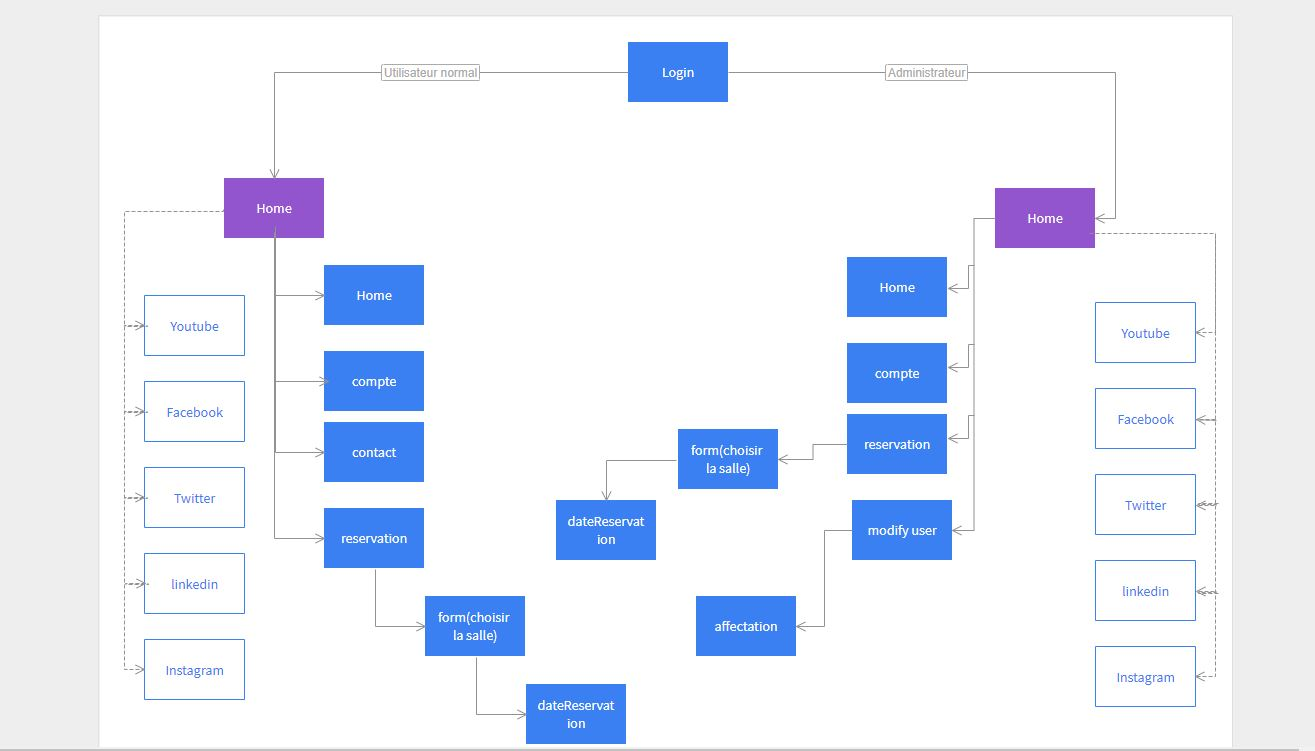
\includegraphics[width=18cm,height=10cm]{img/map.jpg}}
               
               
               
               
                \vspace{1.6cm}
                 \item \textcolor{amethyst}{Installation de la base de données}.
           \vspace{0.4cm}
           
           
            \setlength{\parindent}{1cm}  J'ai installé logiciel xampp. Ce logiciel permet de mettre en place un serveur Web local et un serveur de Base de donnée. Après avoir réalisé le \textcolor{blue}{modèle entité-association}, j'ai créé ma base de données qui est présentée dans l'image suivante :
            
            
            
            \hspace*{-1.05in}
               \noindent\makebox[\textwidth]{\includegraphics[width=19cm,height=11cm]{img/dataBase.png}}
         
         
	 \vspace{1cm}
	 
	 \begin{enumerate}
	 \item \textcolor{red}{\large Tables :}
	 
	 
	 
	 Dans la base de données, il y a six tableaux:
	 
	  \begin{enumerate}
	  
	  \vspace{1cm}
	 
	  \item \textcolor{red}{Salle :} 
	  \vspace{1cm}
	  	Le premier tableau contient les salles
	  	
	  	 \hspace*{-1.05in}
               \noindent\makebox[\textwidth]{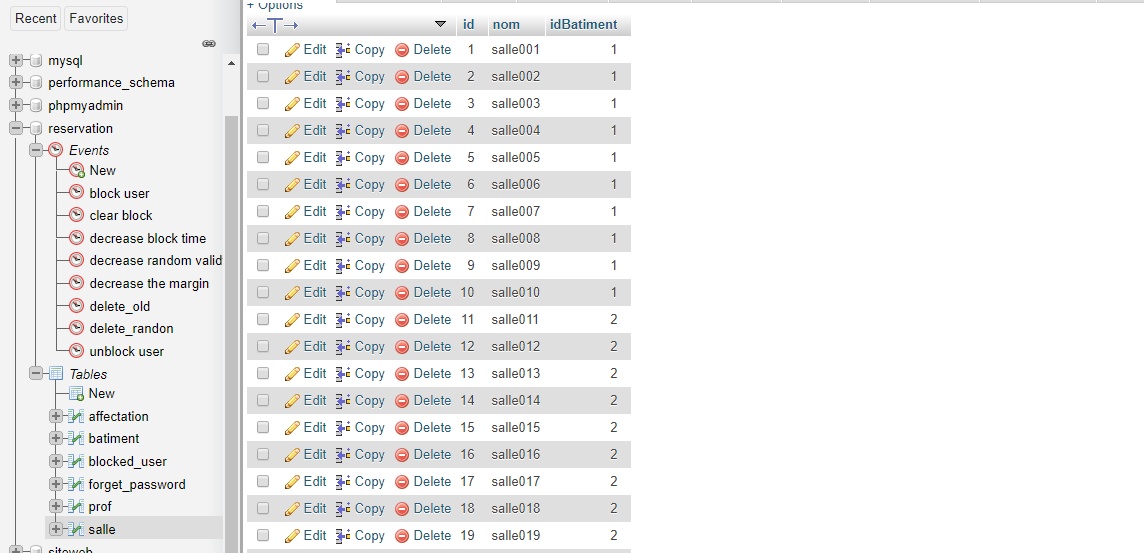
\includegraphics[width=19cm,height=9cm]{img/salle-table.png}}
	  	
	  \vspace{1cm}
	  	
	  \item \textcolor{red}{Batiment :}
	  
	  Le deuxième tableau contient les batiments :
	  
	  \vspace{1cm}
	  
	   \hspace*{-1.05in}
               \noindent\makebox[\textwidth]{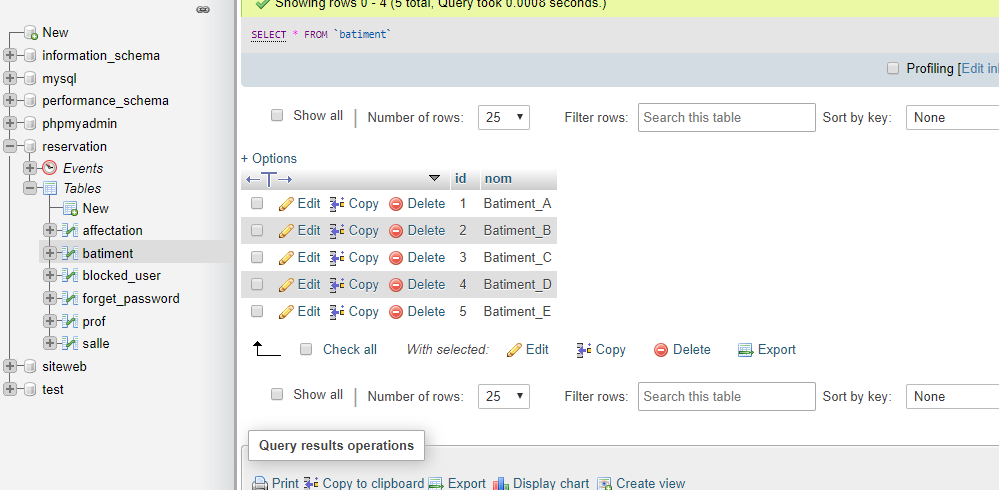
\includegraphics[width=19cm,height=9cm]{img/batiment-table.png}}
	  
	  
	  
	  \vspace{1cm}
	  \item \textcolor{red}{Prof :}
	  
		Le troisième tableau contient les informations des utilisateurs :	  
		
		\vspace{1cm}		
		
		\hspace*{-1.05in}
               \noindent\makebox[\textwidth]{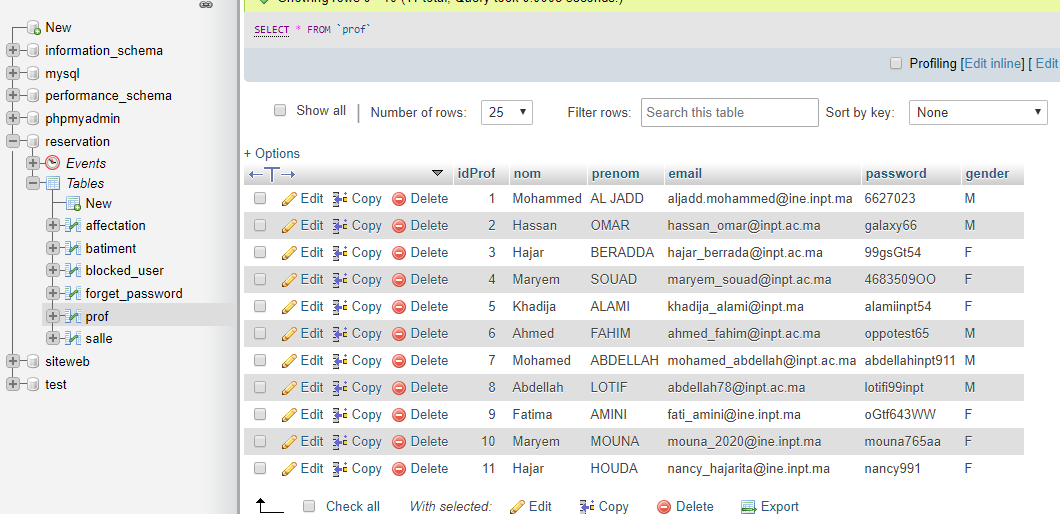
\includegraphics[width=19cm,height=9cm]{img/prof-table.png}}		
		
		
	  
	  
\vspace{3cm}	  
	  
	  \item \textcolor{red}{Affectation :}
	  
	  Le quatrième tableau contient toutes les réservations qui ont été faites :	 
	  
	  \vspace{1cm} 
		
		\hspace*{-1.05in}
               \noindent\makebox[\textwidth]{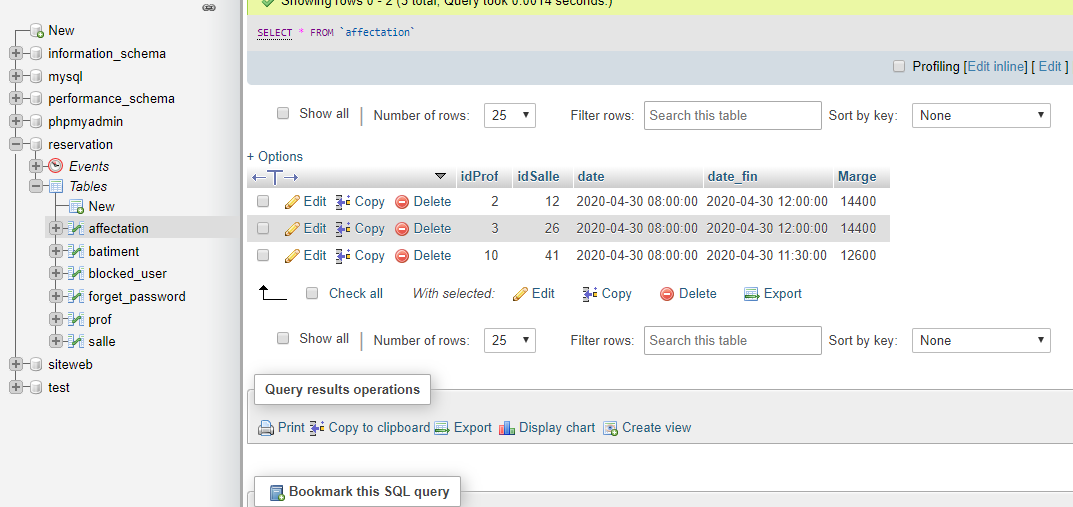
\includegraphics[width=19cm,height=9cm]{img/affectation-table.png}}
	  
	  
	  \vspace{1cm}
	  
	  \item \textcolor{red}{Forget-password :}
	  
		Ce tableau contient le code envoyé pour la réinitialisation du mot de passe :	
		\vspace{1cm}  
		
		\hspace*{-1.05in}
               \noindent\makebox[\textwidth]{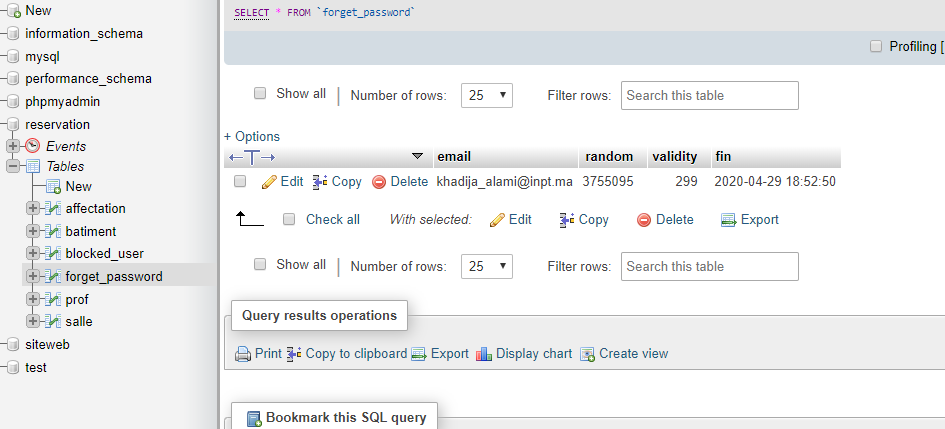
\includegraphics[width=19cm,height=9cm]{img/reset-table.png}}	  
	  
	  \vspace{3cm}
	  	
	  \item \textcolor{red}{Bloqued-user :}
	 
	 La table Lost contient les utilisateurs qui n'ont pas réussi à entrer le bon code, bloqué ou non :
	 \vspace{1cm}
	 
	 \hspace*{-1.05in}
               \noindent\makebox[\textwidth]{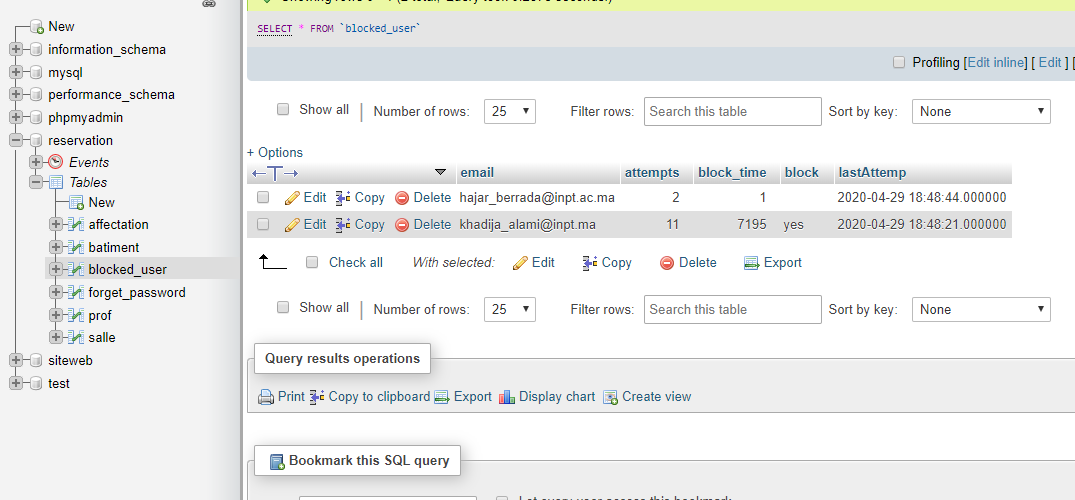
\includegraphics[width=19cm,height=9cm]{img/block-table.png}}	
	 
	 
	 
	 
	 
	 
	 
	  \end{enumerate}
	 
	 
	 
	 \vspace{3cm}
	 
	 
	 \item \textcolor{red}{\large Events :}	 
	 
	 
	 
           
           
            \setlength{\parindent}{1cm} supposons qu'une salle soit réservée pour les prochaines 48 heures, si un utilisateur souhaite la réserver, il doit attendre que la première réservation est terminée, mais grâce à un événement (\textcolor{red}{event}) dans la base de données, la durée de la réservation diminue automatiquement lorsque l'heure de la réservation est venue, donc quand une heure s'est écoulée, la salle peut être réservée car l'utilisateur a le droit de réserver au moins une heure .
            \vspace{1.25cm}
            
            \setlength{\parindent}{1cm} Il y a huit événements \textcolor{red}{Event} dans la base de données, chacun est expliqué ci-dessous avec des images.\\
	\textcolor{red}{Database event} :  
	
	\begin{enumerate}
	\item \textcolor{blue}{Diminuer la durée de la réservation}
	\item \textcolor{blue}{Supprimer les anciennes réservations}
	\item \textcolor{blue}{Diminuer le temps de validité du code de réinitialisation du mot de passe}
	\item \textcolor{blue}{Expirer du code de réinitialisation du mot de passe}
	\item \textcolor{blue}{Bloquer les utilisateurs}
	\item \textcolor{blue}{Diminuer le temps de blocage}
	\item \textcolor{blue}{Débloquer les utilisateurs}
	\item \textcolor{blue}{Effacer les tentatives infructueuses après une heure des dernières tentatives}

	\end{enumerate}
	
	\vspace{2cm}
	
	
	Cet événement diminuera la durée de la réservation quand il commencera :      
         
         \hspace*{-1.05in}
               \noindent\makebox[\textwidth]{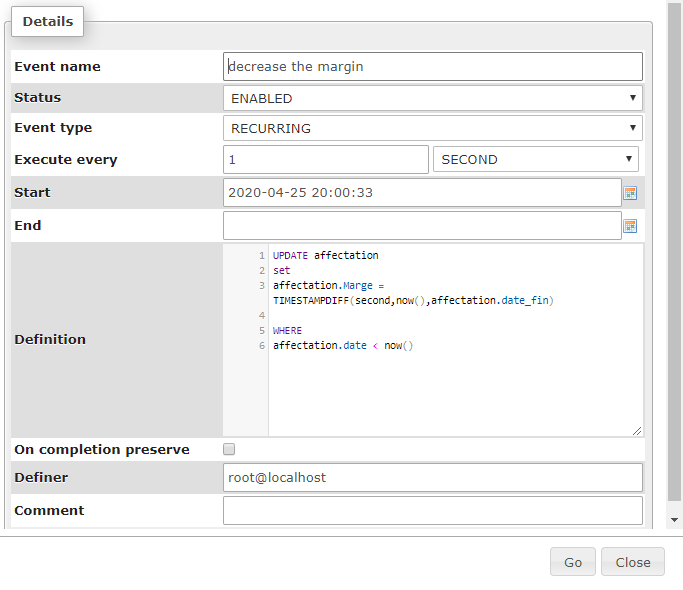
\includegraphics[width=14cm,height=11cm]{img/decrease-margin.png}}
         
         
         Un autre événement dans la base de données va supprimer toute réservation terminée :
         
		\hspace*{-1.05in}
               \noindent\makebox[\textwidth]{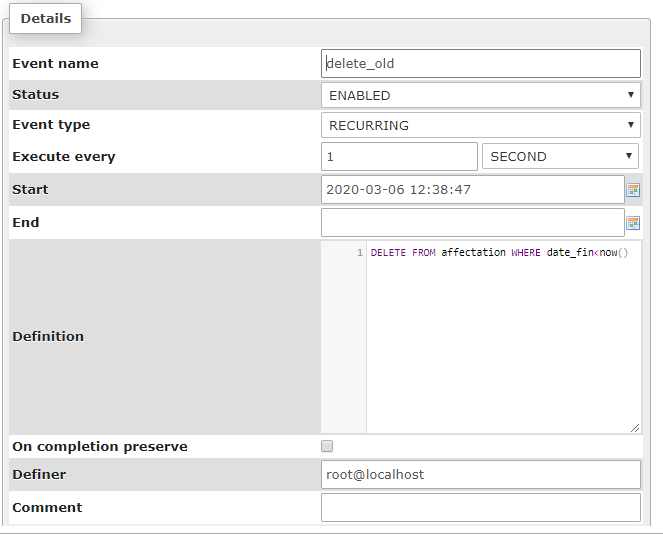
\includegraphics[width=14cm,height=9.5cm]{img/old-reservation.png}}         
         
         
         \vspace{4cm}
         
          Cet événement consiste à diminuer une variable 'validity' :
          \vspace{0.5cm}
         
		\hspace*{-1.05in}
               \noindent\makebox[\textwidth]{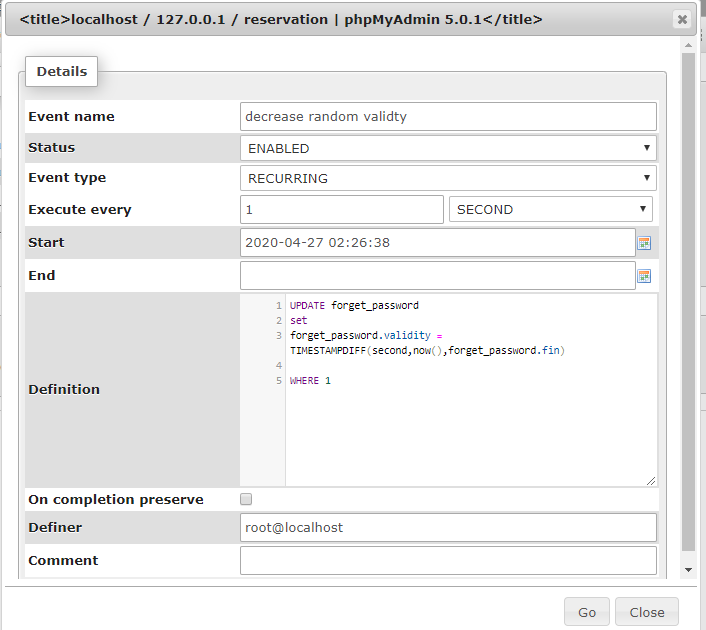
\includegraphics[width=14cm,height=9.5cm]{img/decrease-random-validty.png}}
               \vspace{1cm}
                Lorsque la variable est égale à zéro, l'événement suivant supprimera la ligne de la table car le code envoyé aura expiré après 5 minutes :
                
         \vspace{0.5cm}

		\hspace*{-1.05in}
               \noindent\makebox[\textwidth]{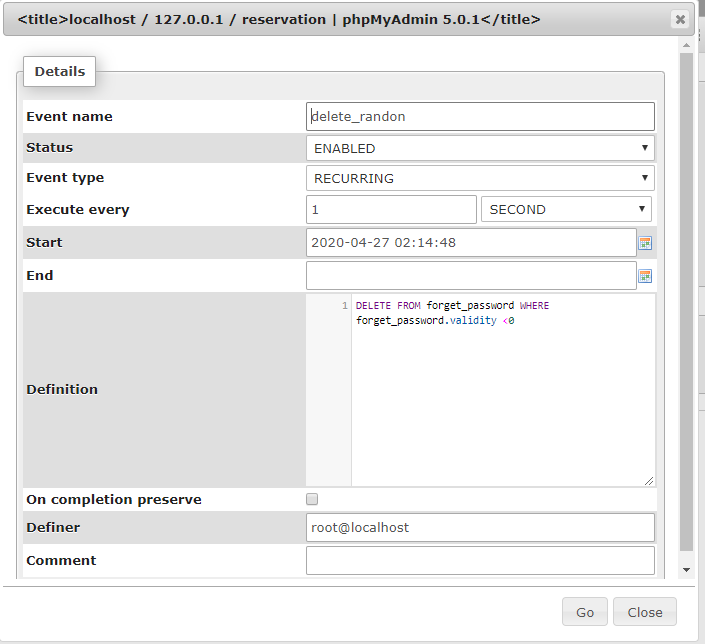
\includegraphics[width=14cm,height=9.5cm]{img/delete_randon.png}}
  \newpage       
        
        Un événement définira la colonne de blocage sur 'yes', ce qui signifie que l'utilisateur est bloqué pour la réinitialisation du mot de passe et le dernier code envoyé sera expiré just après :
        
        \vspace{0.4cm}
        \hspace*{-1.05in}
               \noindent\makebox[\textwidth]{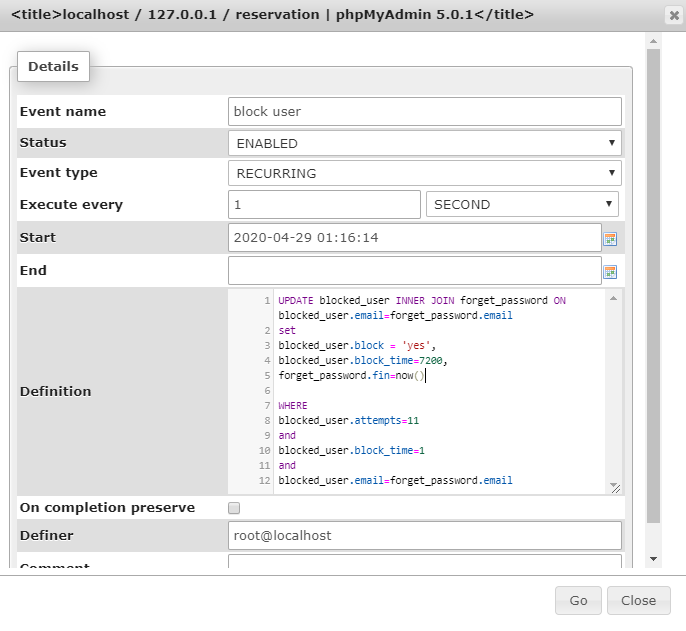
\includegraphics[width=14cm,height=8.5cm]{img/block-user.png}}
        
        
       Après avoir empêché un utilisateur de réinitialiser le mot de passe, un e-mail sera envoyé à son e-mail pour savoir si celui qui tentait de réinitialiser son mot de passe pour l'aider à en obtenir un nouveau :
        
        \vspace{0.4cm}
        \hspace*{-1.05in}
               \noindent\makebox[\textwidth]{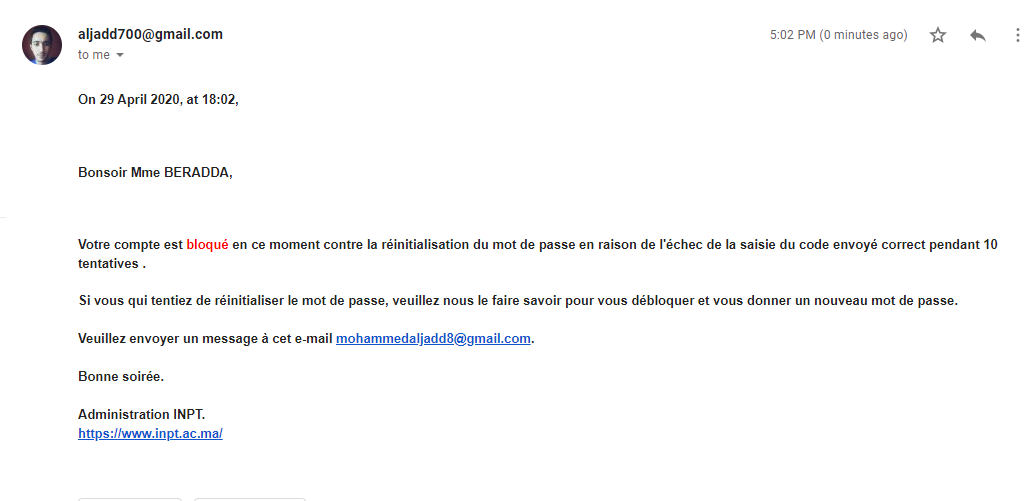
\includegraphics[width=17cm,height=8.5cm]{img/block-gmail.png}}
        
        
        
        \newpage
        
         Un événement décrémente le temps de blocage :
        
        \vspace{0.4cm}
        \hspace*{-1.05in}
               \noindent\makebox[\textwidth]{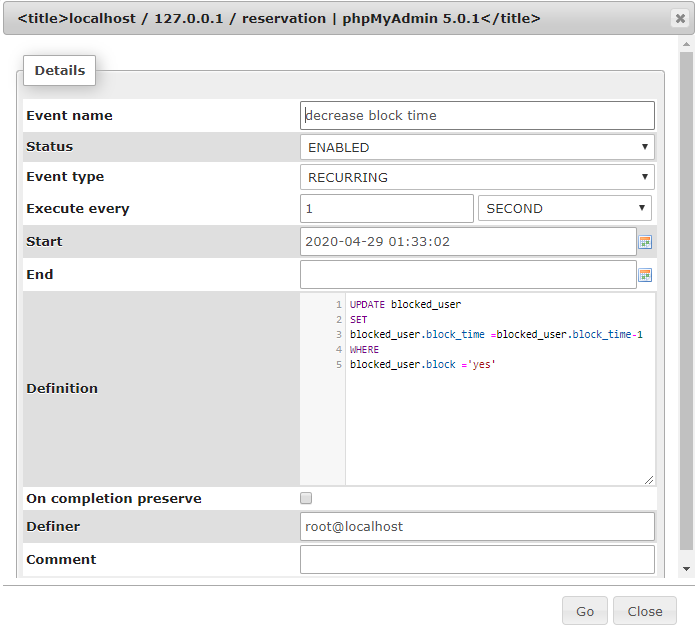
\includegraphics[width=14cm,height=8.5cm]{img/decrease-block-time.png}}
        
        Un événement débloquera l'utilisateur :
        
        \vspace{0.4cm}
        \hspace*{-1.05in}
               \noindent\makebox[\textwidth]{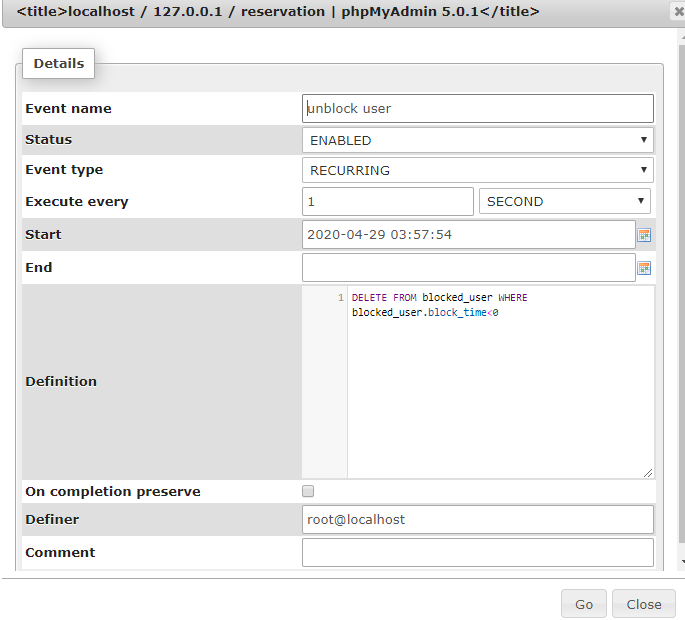
\includegraphics[width=14cm,height=8.5cm]{img/unblock-user.png}}
        
        \newpage
        Un événement supprimera un utilisateur du tableau des utilisateurs bloquants si les dernières tentatives datent d'une heure :
        
        \vspace{0.4cm}
        \hspace*{-1.05in}
               \noindent\makebox[\textwidth]{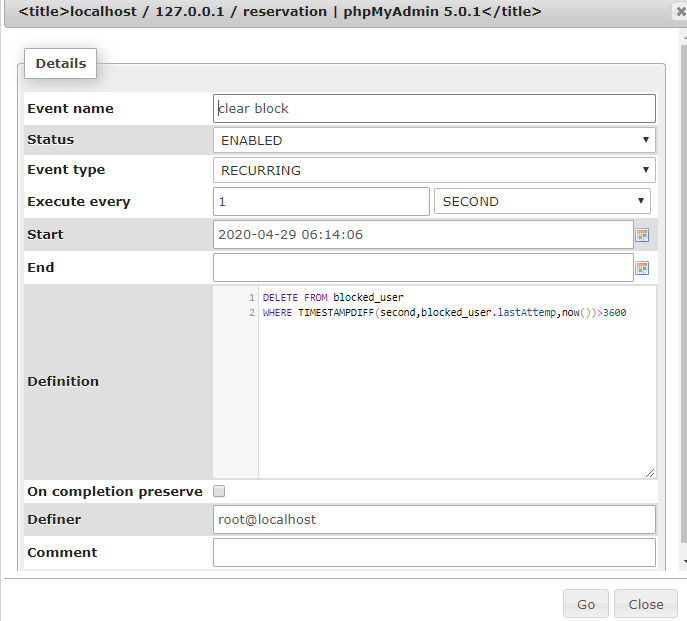
\includegraphics[width=14cm,height=8.5cm]{img/clear-block.png}}
        
        
        
        
        
         \end{enumerate}
        
        
        
        
        
         \item \textcolor{amethyst}{Créer des maquettes}.
         
         \vspace{0.4cm}
                \setlength{\parindent}{1cm} J'ai créé des maquettes pour mon site Web en utilisant le site Web \textcolor{blue}{moqups.com}. Ils maquettes sont présentés dans le dossier maquettes.
         
\hspace*{-1.05in}
               \noindent\makebox[\textwidth]{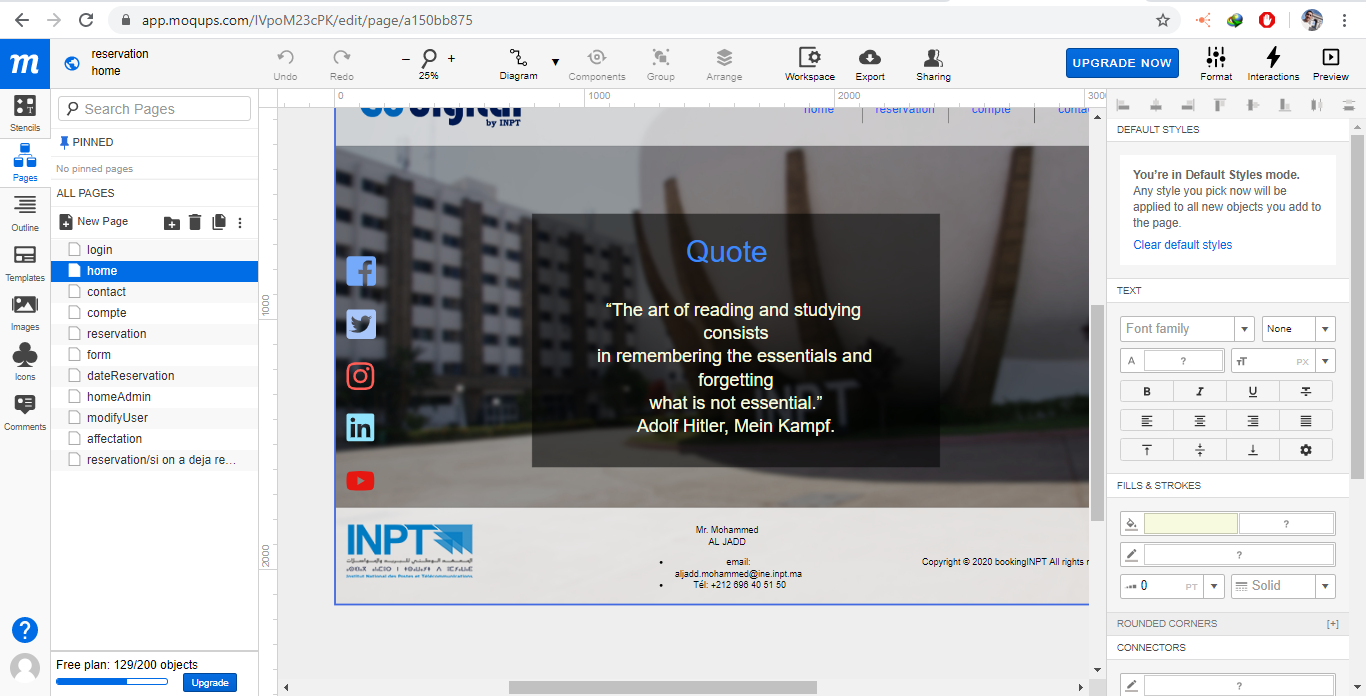
\includegraphics[width=18cm,height=8cm]{img/moqups.png}}         
         \vspace{1cm}
         \item \textcolor{amethyst}{Apprenez \textbf{GITHUB}}.
         
         \vspace{0.4cm}
                \setlength{\parindent}{1cm} J'ai regardé un video sur youtube pour apprendre comment commiter du \textcolor{blue}{VISUAL STUDIO CODE}, créer un project \textcolor{blue}{basic KANBAN}.
         \newpage
         \item \textcolor{amethyst}{Créer des pages WEB}.
         
         \vspace{0.4cm}
                \setlength{\parindent}{1cm} J'ai commencé à créer des pages Web \textcolor{blue}{\textbf{PHP}}. Après que je termine une page, je crée une page \textcolor{blue}{\textbf{CSS}} pour appliquer les style .Mais j'ai respecté la façon que les informations entre par l'utlisateur vont  être traitées dans des pages des différents. Par exemple utilisateur elle veut changer son mot de passe, son nouveau mot de passe va être traité dans une autre page.
         
         \hspace*{-1.05in}
               \noindent\makebox[\textwidth]{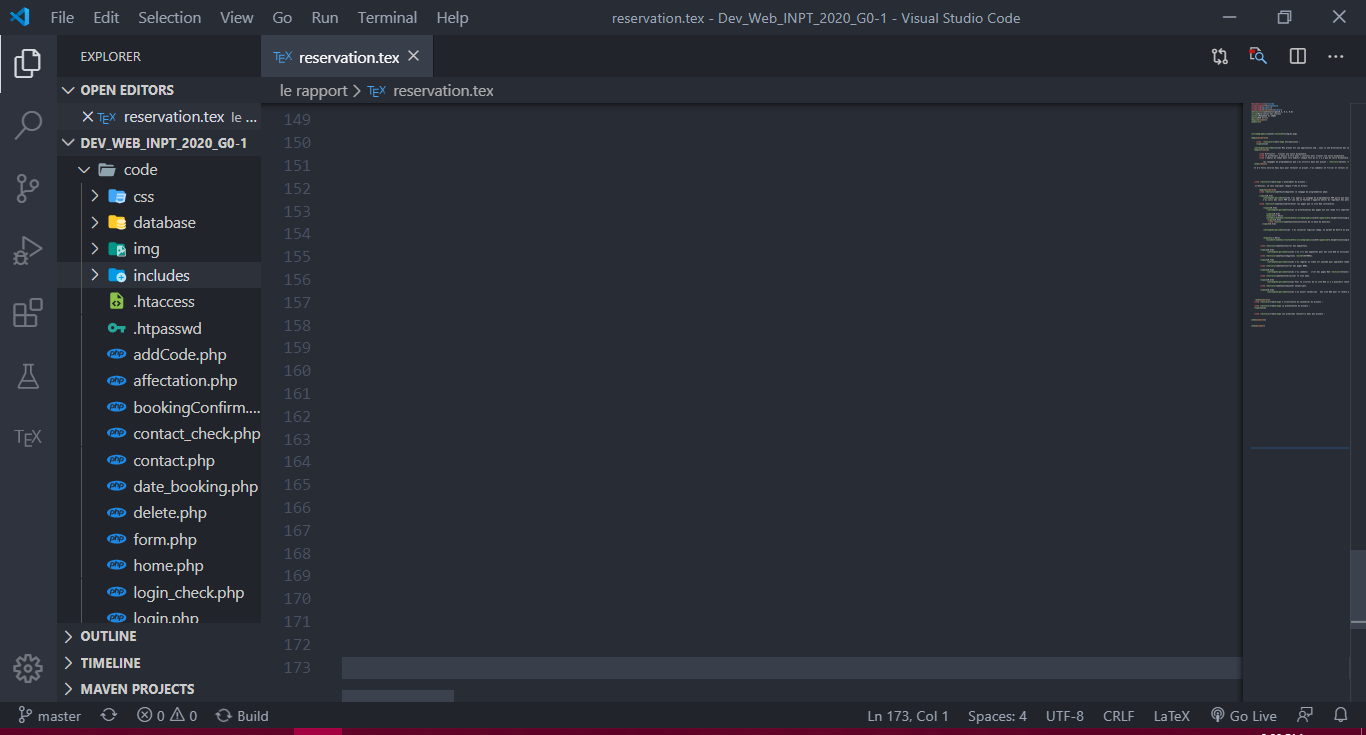
\includegraphics[width=18cm,height=12cm]{img/visual.png}}
         \item \textcolor{amethyst}{Sécuriser le site web}.
         
         \vspace{0.4cm}
                \setlength{\parindent}{1cm} Pour la sécurité de ce site Web il y a plusieurs choses que j'ai fait. La première chose est d'empêcher l'accès à certaines pages sans connexion. Une deuxième chose est d'empêcher l'accès à certains car ils sont destinés à l'administrateur même en cas de connexion.
         
         \item \textcolor{amethyst}{Ajouter JavaScript}.
         
         \vspace{0.4cm}
                \setlength{\parindent}{1cm} J'ai ajouté JavaScript à mon site Web pour le rendre plus dynamique, par exemple, lorsqu'il y a des erreurs comme si l'utilisateur n'a pas entré ses informations et soumis, le site Web affichera une erreur indiquant que les champs sont vides à l'aide de la boîte d'alerte.
         
         
         \vspace{4cm}
         \vspace{4.2cm}
   
    \end{enumerate}
   \item \textcolor{red}{\huge L'illustration du calendrier du projet} :  
   \vspace{1.2cm}
   
         \hspace*{-1.2in}
        \begin{tabular}{|c | c | c|}
        \hline
          \textcolor{red}{\Large La tâche} & \textcolor{red}{\Large date de début} & \textcolor{red}{\Large date de fin}\\ 
        \hline
        Apprenez le langage de programmation \textcolor{blue}{\textbf{PHP}} & 2020/02/22 & 2020/02/28 \\ 
        \hline
        Déterminer les pages que le site Web contiendra & 2020/02/29 & 2020/02/30 \\ 
        \hline
        Installation de \textcolor{red}{la base de données} & 2020/03/15 & 2020/03/20\\
        \hline
        Créer \textcolor{red}{des maquettes} & 2020/04/01  & 2020/04/01\\
        \hline
        Apprenez \textcolor{blue}{\textbf{GITHUB}} & 2020/04/02  & 2020/04/03\\
        \hline
        Créer des pages WEB & 2020/04/04  & 2020/05/06\\
        \hline
        Essayez le site et assurez-vous qu'il fonctionne bien & 2020/04/04  & 2020/05/06\\
		\hline        
        Sécuriser le site web & 2020/04/04  & 2020/04/29\\
        \hline
        Ajouter \textcolor{blue}{\textbf{JavaScript}} & 2020/04/06  & 2020/05/06\\
        \hline
        Création d'événements (\textcolor{red}{events}) dans la base de données & 2020/04/25 & 2020/04/29\\
        \hline
         Création d'\textcolor{red}{un système de mot de passe oublié} & 2020/04/26 & 2020/04/27\\
        \hline
        Créer des maquettes pour le système de mot de passe oublié & 2020/04/27  & 2020/04/28\\
        \hline
        Empêcher l'utilisateur de réinitialiser le mot de passe après \textcolor{red}{10 tentatives infructueuses} & 2020/04/29  & 2020/04/29\\
        \hline
        \end{tabular}
        
        \vspace{1cm}
  
        
        
        
        
        
        
   \vspace{1cm}
   \item \textcolor{red}{\huge La presentation du projet} :  
   \vspace{0.7cm}
   

	Lorsque vous entrez sur le site, la première page qui apparaît est la page de connexion
	
	\hspace*{-0.7in}
               \noindent\makebox[\textwidth]{
\includegraphics[width=18.8cm,height=8.5cm]{img/login.png}}
               
               
               
               \newpage
               
               
    Si vous cliquez sur le bouton Soumettre et en laissant un champ vide, la boîte d'alerte apparaîtra comme l'image suivante montrant :
   \vspace{0.7cm}
   
\hspace*{-0.7in}

               \noindent\makebox[\textwidth]{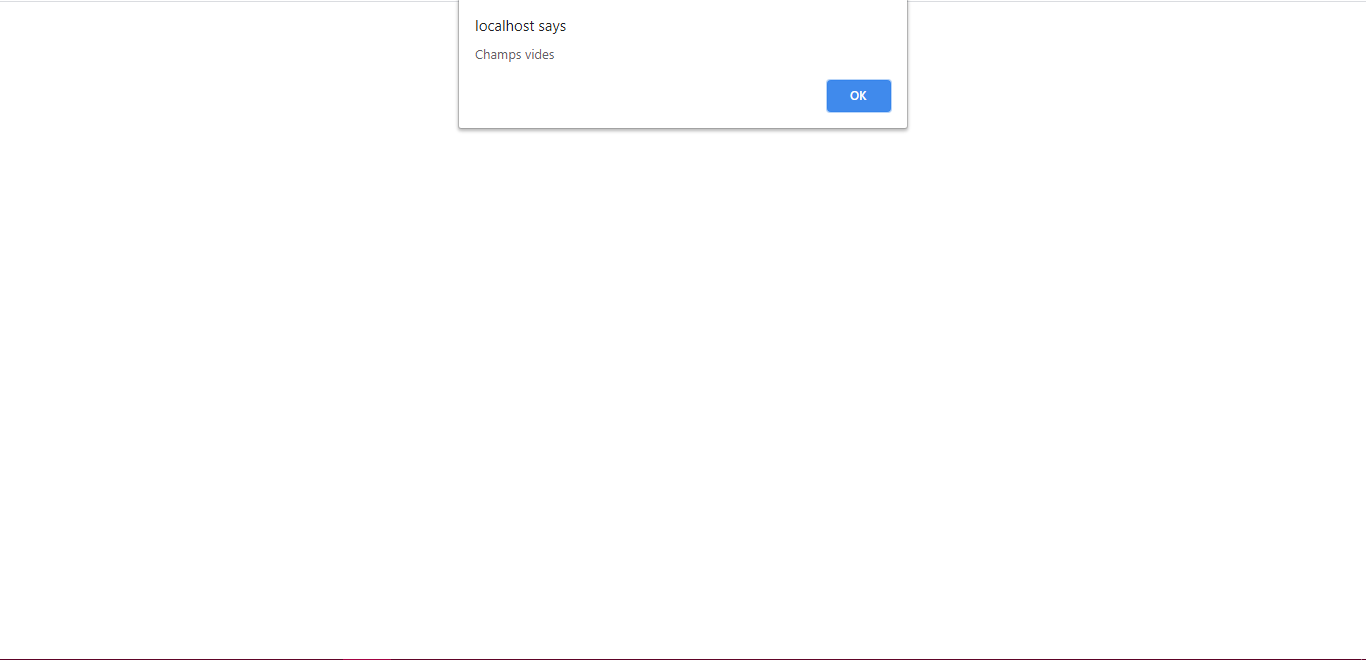
\includegraphics[width=\paperwidth,height=8.5cm]{img/login-empty-fileds.png}}

Si vos informations étaient erronées, la boîte d'alerte indiquera:

\vspace{0.4cm}
   
\hspace*{-0.7in}

               \noindent\makebox[\textwidth]{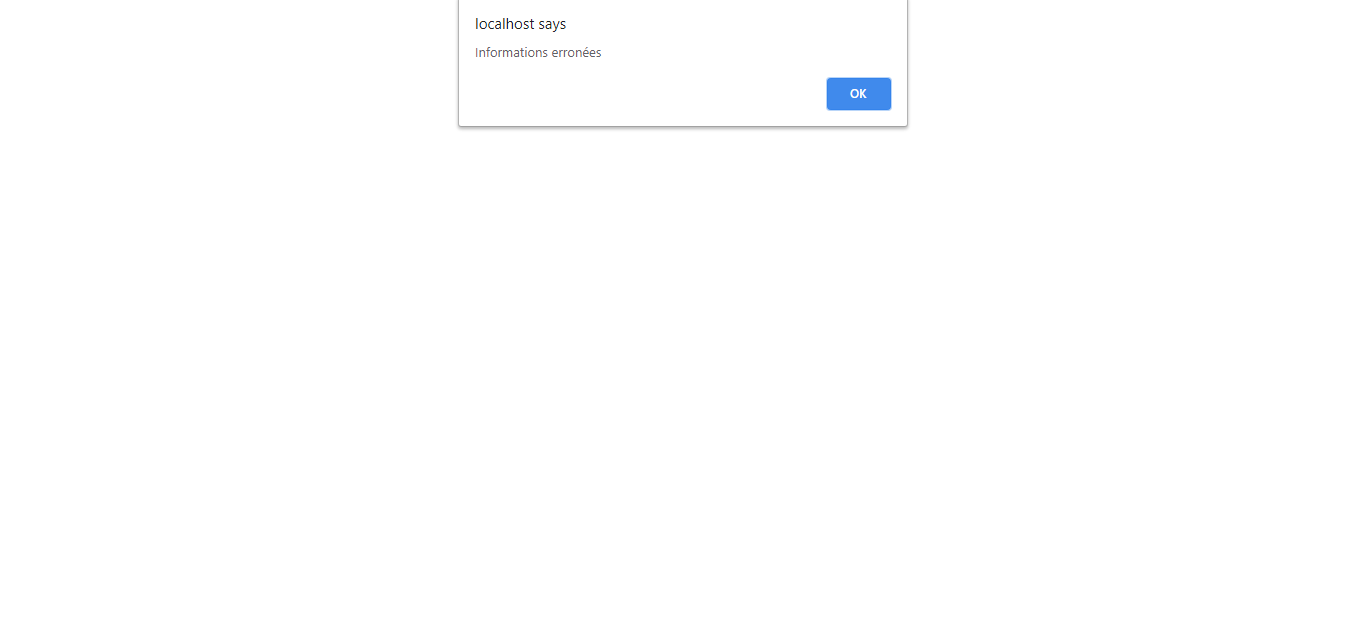
\includegraphics[width=\paperwidth,height=6.5cm]{img/login-wrong-infos.png}}

\newpage
	Si l'utilisateur oublie le mot de passe, il cliquera sur le lien en bas du page de login. Une page va apparaitre comme le montre l'image suivante.

\vspace{0.4cm}
\hspace*{-0.7in}
               \noindent\makebox[\textwidth]{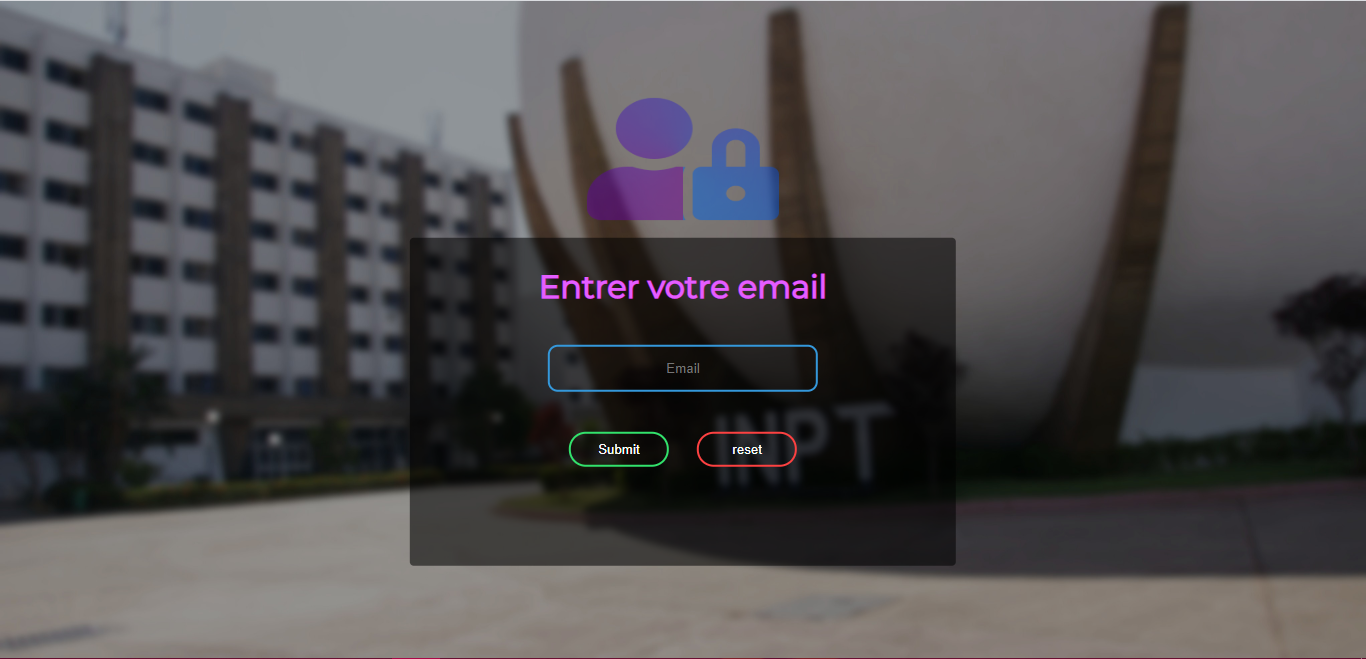
\includegraphics[width=18cm,height=6.5cm]{img/email-reset.png}}


Si l'e-mail entré n'est pas valide :


\vspace{0.4cm}
\hspace*{-0.7in}
               \noindent\makebox[\textwidth]{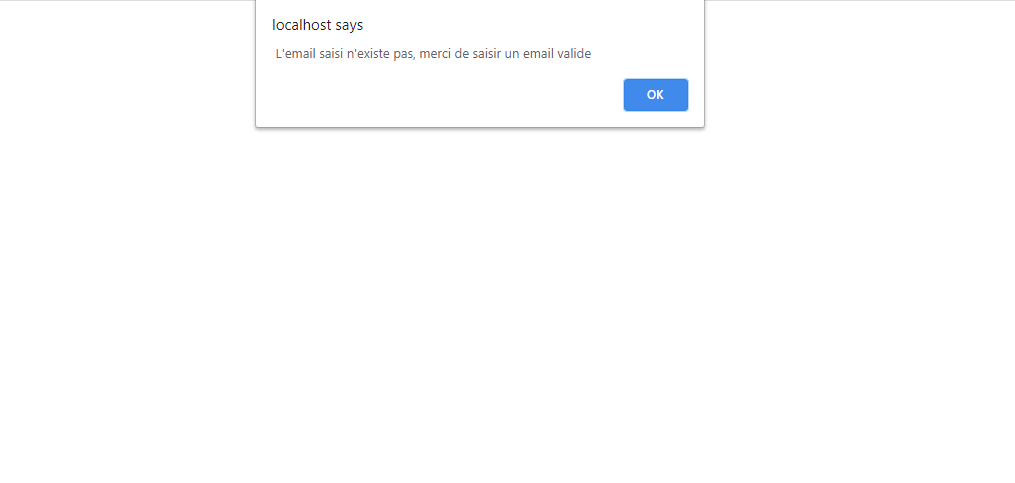
\includegraphics[width=18cm,height=6.5cm]{img/email-reset-incorrect.png}}



Si l'e-mail est entré valide, un code sera envoyé comme le message d'alerte suivant s'affiche:

\vspace{0.4cm}
\hspace*{-0.7in}
               \noindent\makebox[\textwidth]{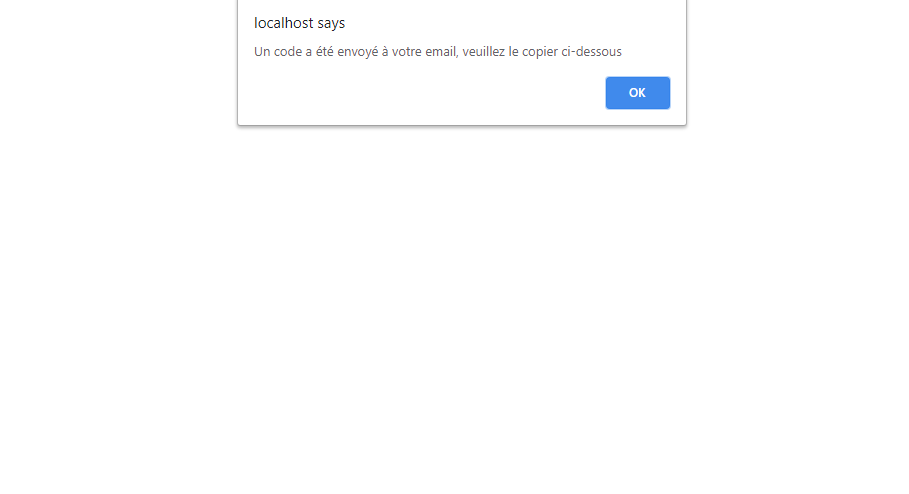
\includegraphics[width=18cm,height=6.5cm]{img/code-sent.png}}

Voici le message qui contient le code envoyé à copier :

\textcolor{red}{NB : Bonsoir/Bonjour et Bonjour/Bonsoir depend du temps accueil. Mme/Mr depend du sexe de l'utilisateur.}


\vspace{0.4cm}
\hspace*{-0.7in}
               \noindent\makebox[\textwidth]{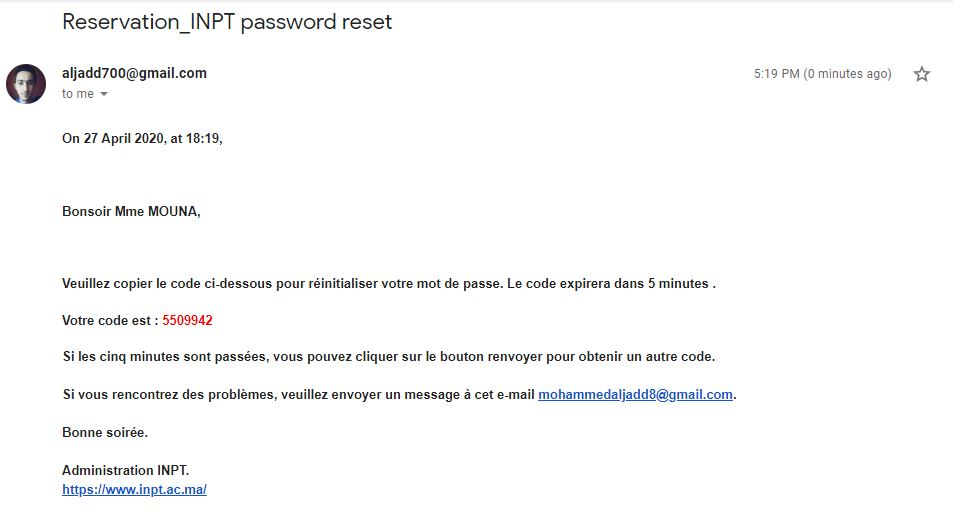
\includegraphics[width=18cm,height=8.5cm]{img/code-gmail.jpg}}


Voila la page pour entrer le code :

\vspace{0.4cm}
\hspace*{-0.7in}
               \noindent\makebox[\textwidth]{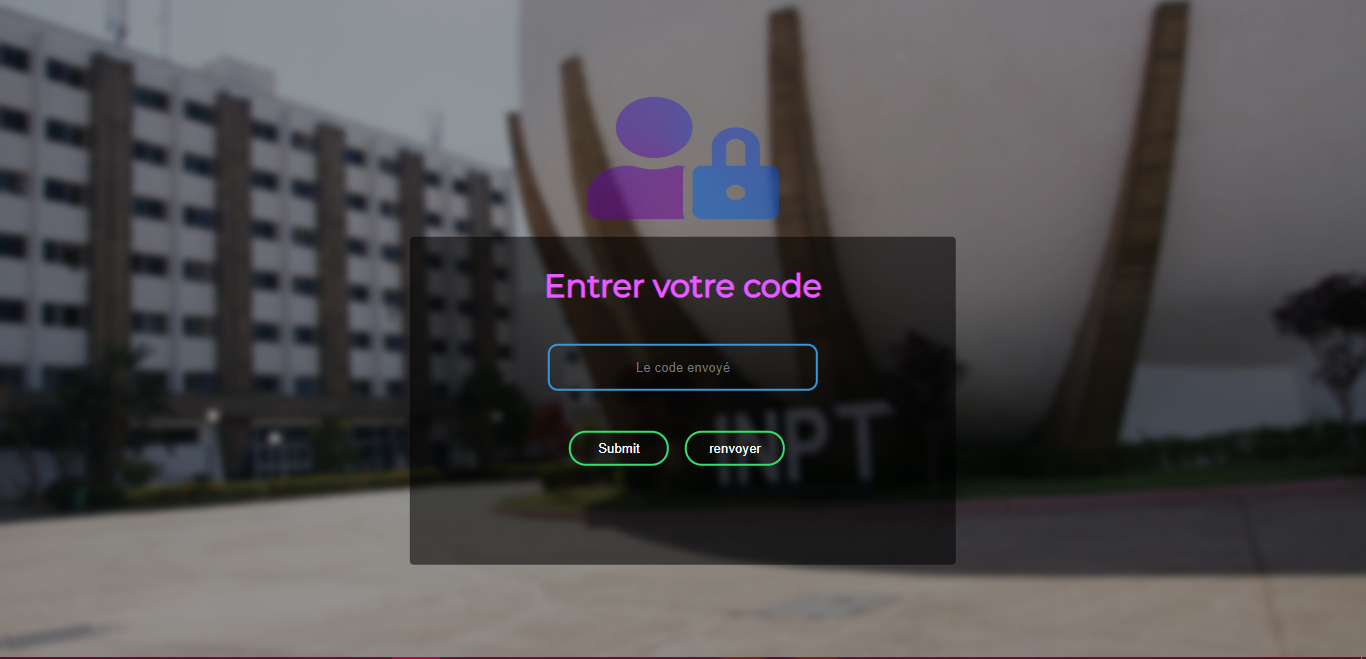
\includegraphics[width=18cm,height=8.5cm]{img/enter-code.png}}




Si le code est incorrect :

\vspace{0.4cm}
\hspace*{-0.7in}
               \noindent\makebox[\textwidth]{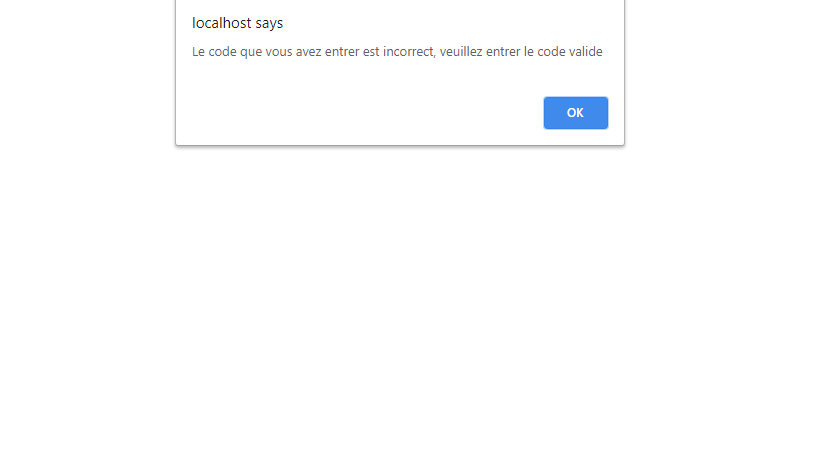
\includegraphics[width=18cm,height=6cm]{img/code-incorrect.png}}
               \newpage
     \vspace{0.4cm}          
       Si le code a expiré :       
               
               
\vspace{0.4cm}
\hspace*{-0.7in}
               \noindent\makebox[\textwidth]{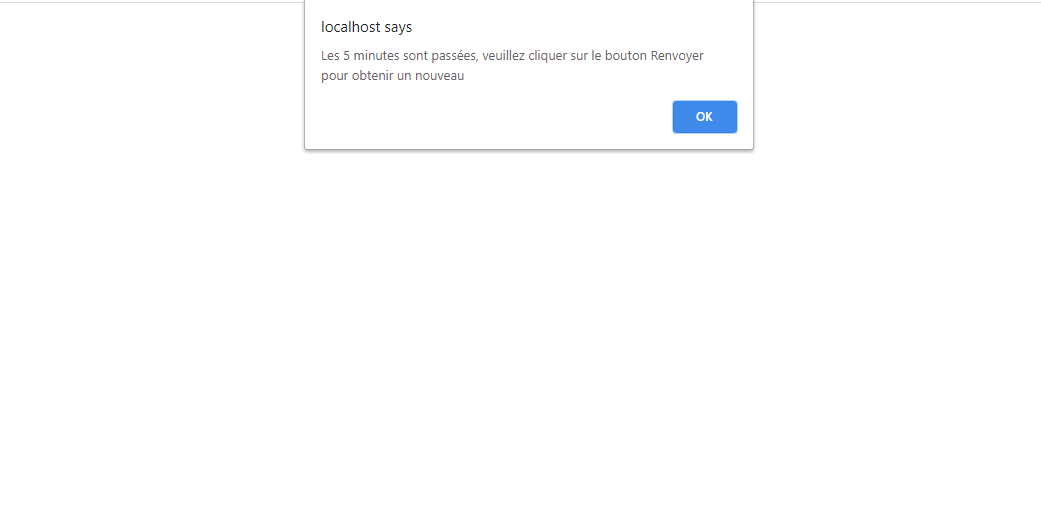
\includegraphics[width=18cm,height=5cm]{img/five-minutes.png}}
            
              
 \vspace{0.4cm}

Mais si l'utilisateur saisit un code 10 fois incorrect, il ne pourra pas réinitialiser ce mot de passe pendant les  \textcolor{red}{2 heures prochaines} :
 
\vspace{0.4cm}
\hspace*{-0.7in}
               \noindent\makebox[\textwidth]{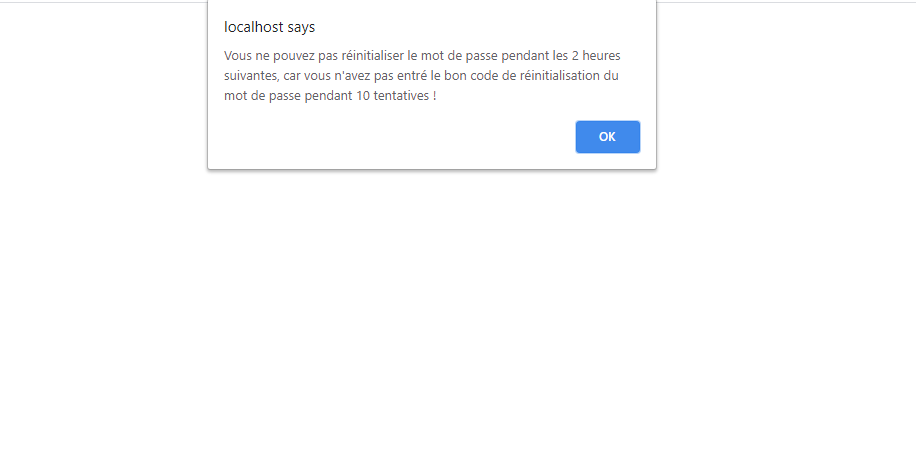
\includegraphics[width=18cm,height=5cm]{img/ten-attempts.png}} 
 
 
 
 
               
Si le code est correct :


\vspace{0.4cm}
\hspace*{-0.7in}
               \noindent\makebox[\textwidth]{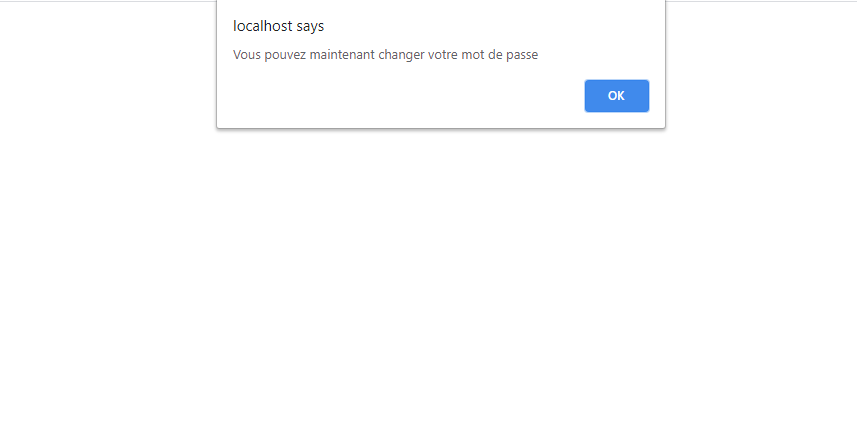
\includegraphics[width=18cm,height=8.5cm]{img/code-correct.png}}

\newpage
Donc une page va apparaitre pour changer le mot de passe :


\vspace{0.4cm}
\hspace*{-0.7in}
               \noindent\makebox[\textwidth]{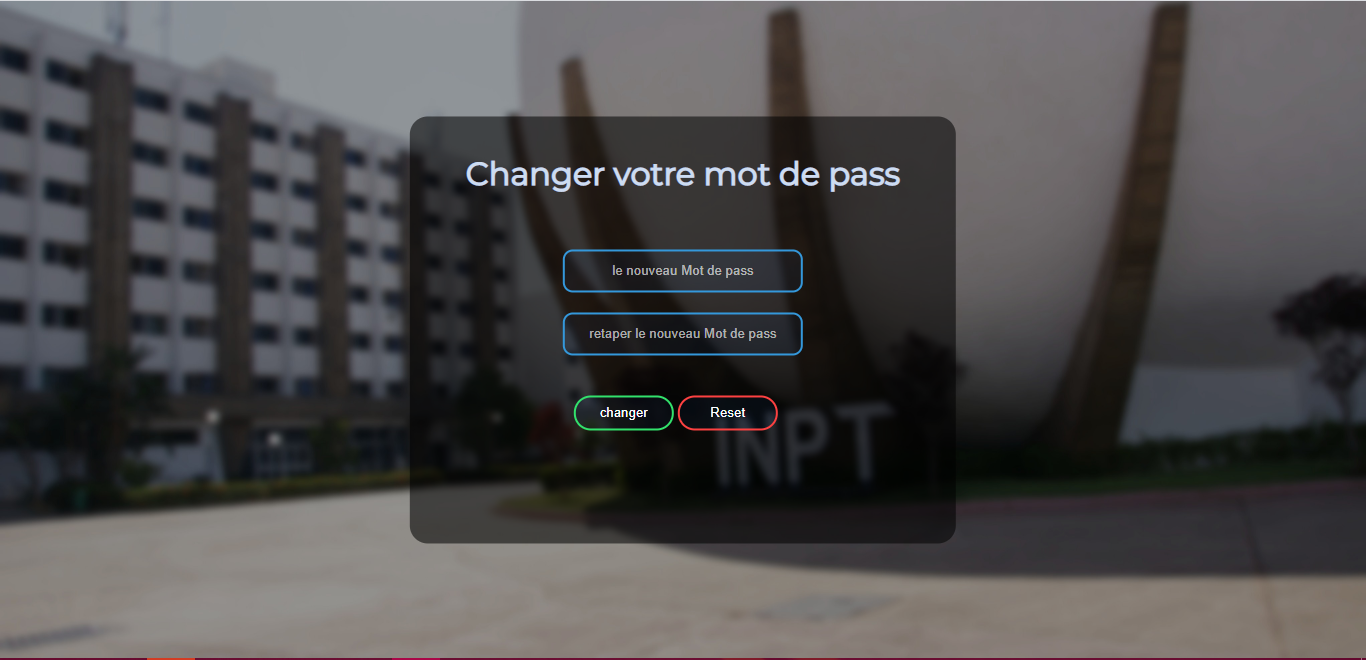
\includegraphics[width=18cm,height=8.5cm]{img/password-reset.png}}
























	Si vos informations étaient correctes, et vous êtes un utilisateur normal, vous serez érigé sur la page d'accueil avec la boîte d'alerte indiquant une formule de salutation avec Mr/Mme cela dépend du sexe de l'utilisateur:



   
   
   
   \hspace*{-0.7in}
               \noindent\makebox[\textwidth]{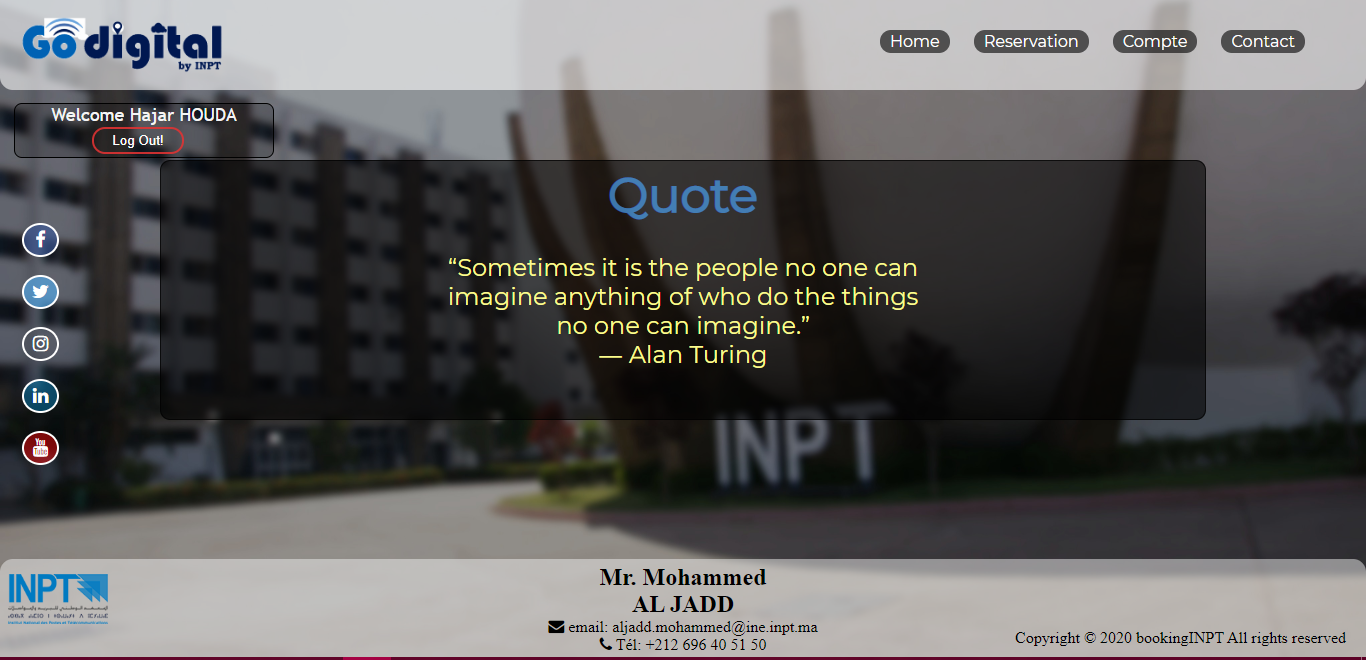
\includegraphics[width=18.8cm,height=8.5cm]{img/home.png}}


\newpage
   La page d'accueil contient une barre de navigation avec 3 autres liens vers d'autres pages.
La première page est la page de contact comme l'image suivante montrant
  
\vspace{0.7cm}
   

   \hspace*{-0.7in}
               \noindent\makebox[\textwidth]{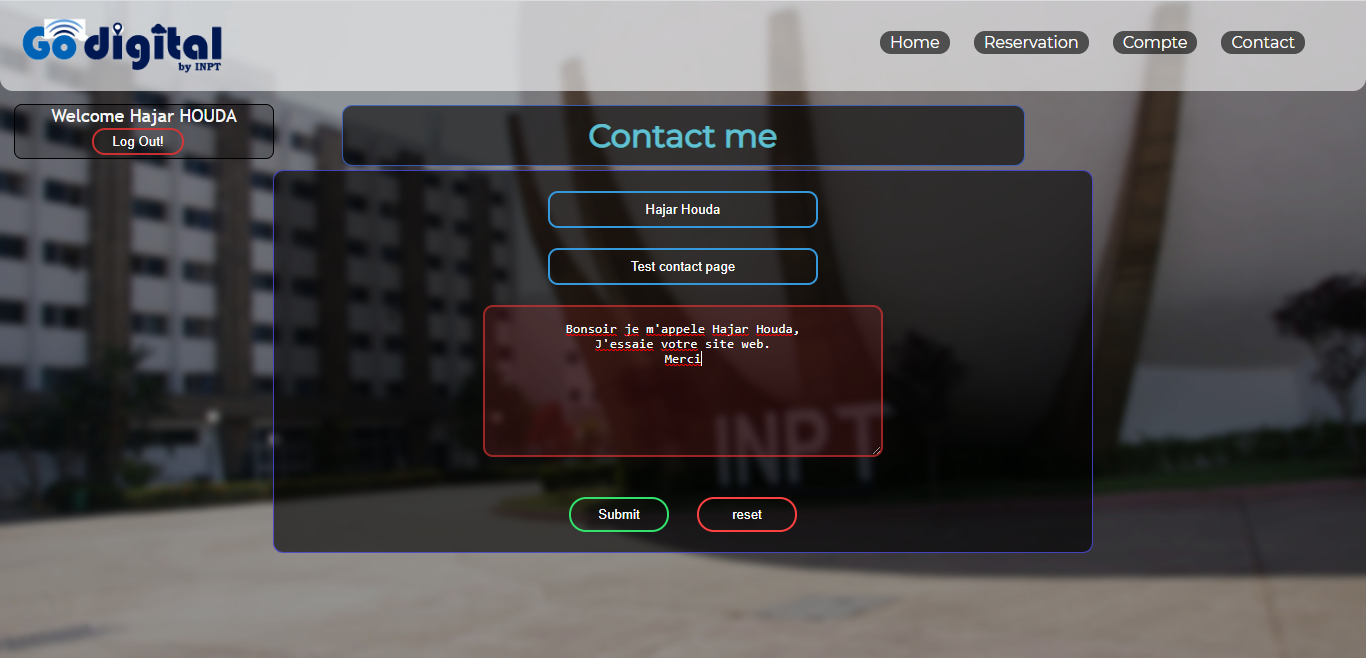
\includegraphics[width=18.8cm,height=8.5cm]{img/contact.png}} 
               
               
Si l'utilisateur souhaite envoyer un message à l'administrateur, un message d'alerte sera le suivant
  
  
  \vspace{0.7cm}
               \hspace*{-0.7in}
               \noindent\makebox[\textwidth]{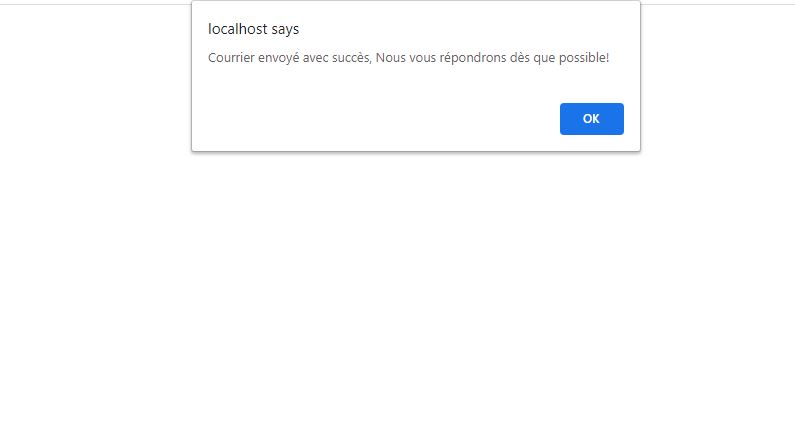
\includegraphics[width=18.8cm,height=8.5cm]{img/courrier-envoye.jpg}} 
  
  
  Et le message serait-il comme suit :
 
   
   
   \vspace{0.7cm}
               \hspace*{-0.7in}
               \noindent\makebox[\textwidth]{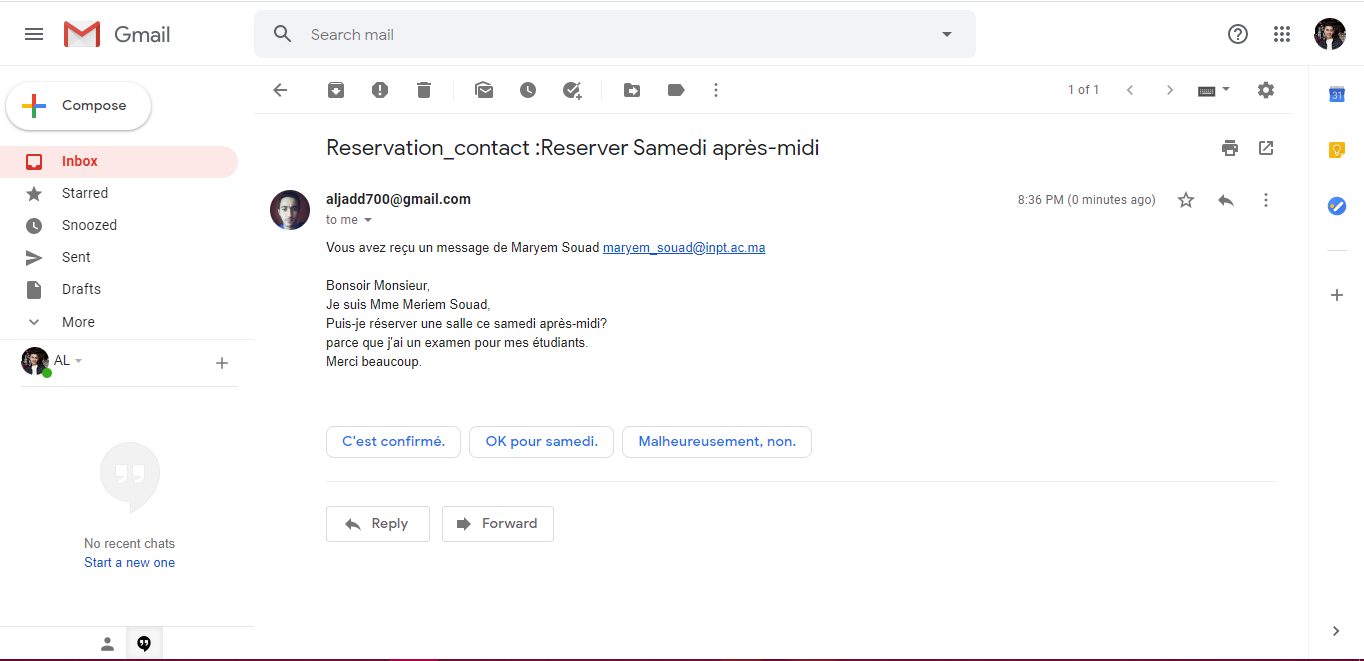
\includegraphics[width=18.8cm,height=8.5cm]{img/courrier-gmail.png}}                
               
               
               
               
               
               Les messages d'alerte sont les mêmes que d'habitude. La deuxième page est la page compte qui permet aux utilisateurs de changer leur mot de passe
  
  \vspace{0.7cm}
   
\hspace*{-0.7in}
               \noindent\makebox[\textwidth]{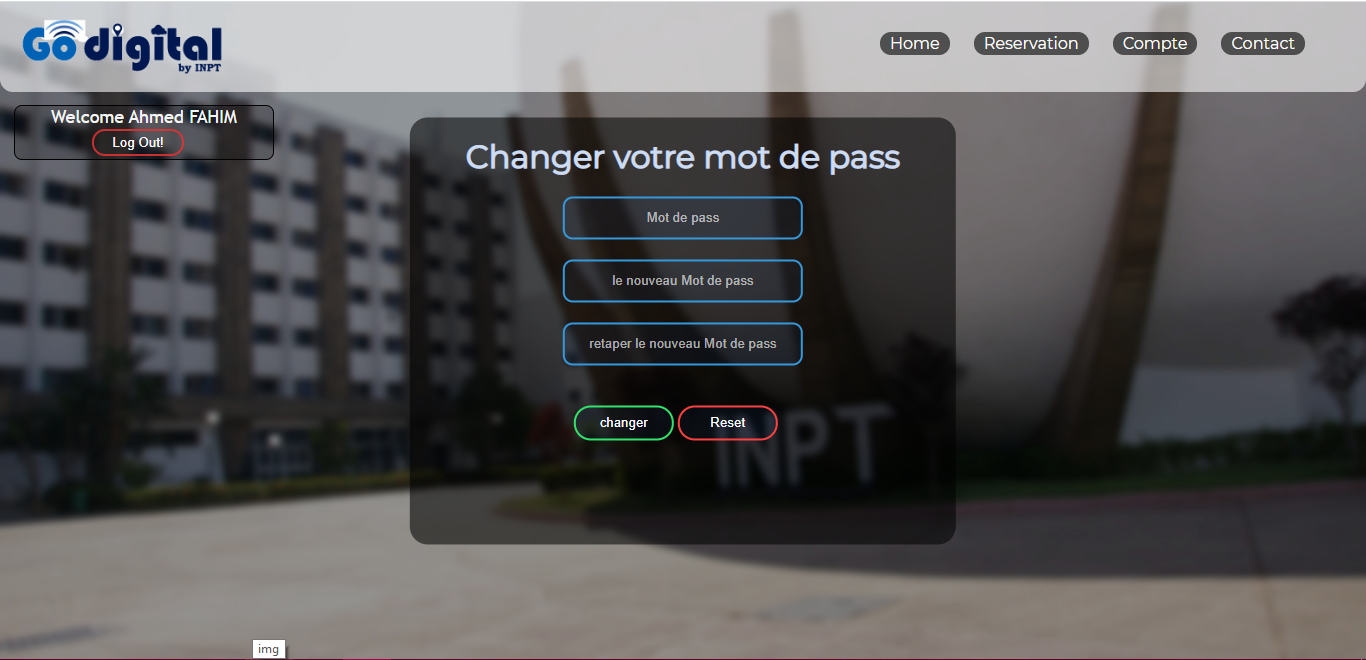
\includegraphics[width=18.8cm,height=8.5cm]{img/password.png}}  
               
 \newpage
  Si les mots de passe étaient erronés, la boîte d'alerte s'affichera comme ci-dessous :
  
   
  \vspace{0.7cm}
   
\hspace*{-0.7in}

               \noindent\makebox[\textwidth]{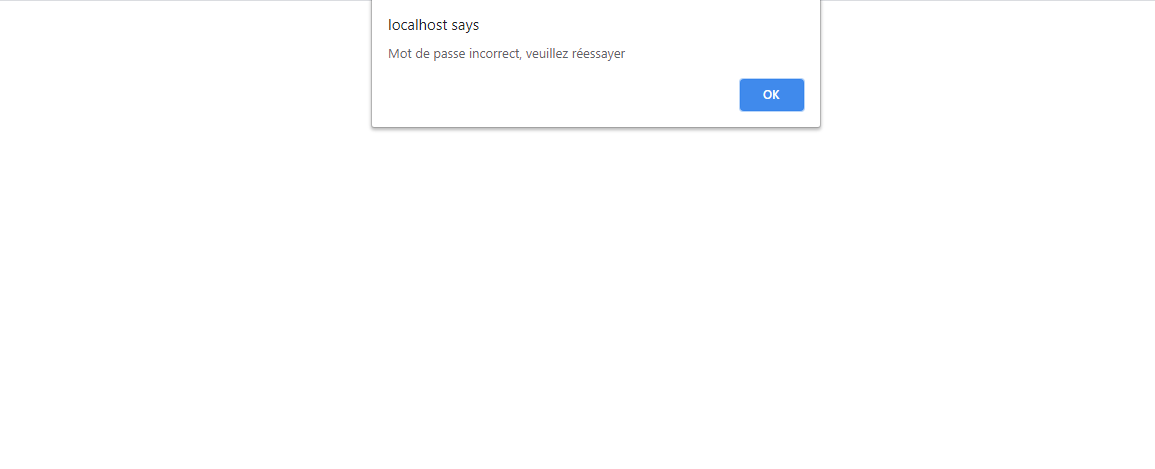
\includegraphics[width=\paperwidth,height=8cm]{img/password-wrong.png}}  
               
  
  
  Si vous entrez correctement votre mot de passe mais que les nouveaux mots de passe ne correspondent pas
  \vspace{0.7cm}
   
\hspace*{-0.7in}

               \noindent\makebox[\textwidth]{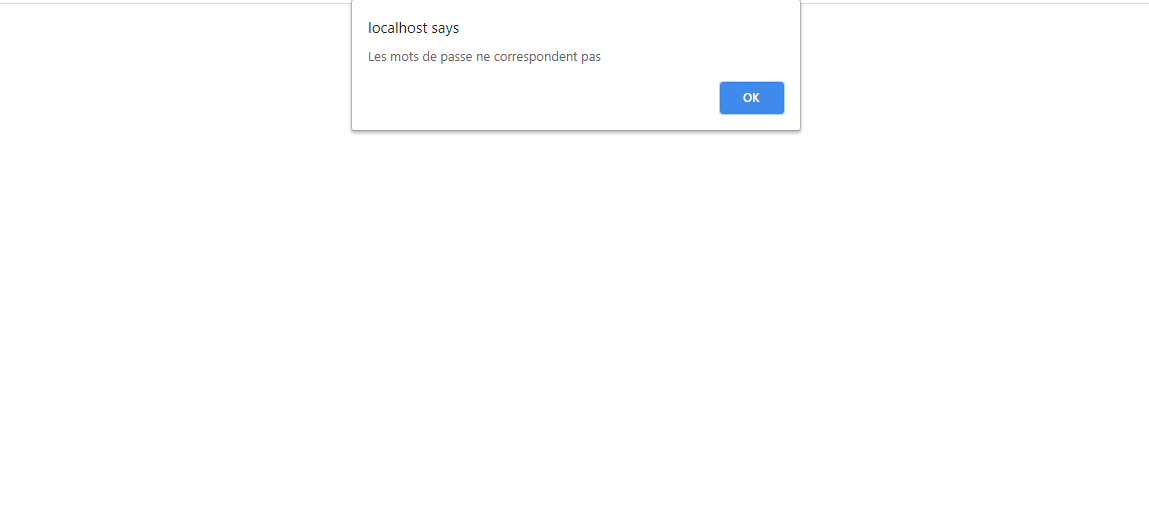
\includegraphics[width=\paperwidth,height=8cm]{img/password-matching.png}}  
               
  
  la page principale de ce projet est la page de réservation. La case du haut contient les batiments avec le nombre de salles disponibles et la case du bas contient des boutons radios  pour choisir le batiment préférable. Les salles disponibles sont celles qui ont au moins \textcolor{red}{une heure} non réservée dans \textcolor{red}{les deux jours prochaines}.
  
  \vspace{0.7cm}
   
\hspace*{-0.7in}
               \noindent\makebox[\textwidth]{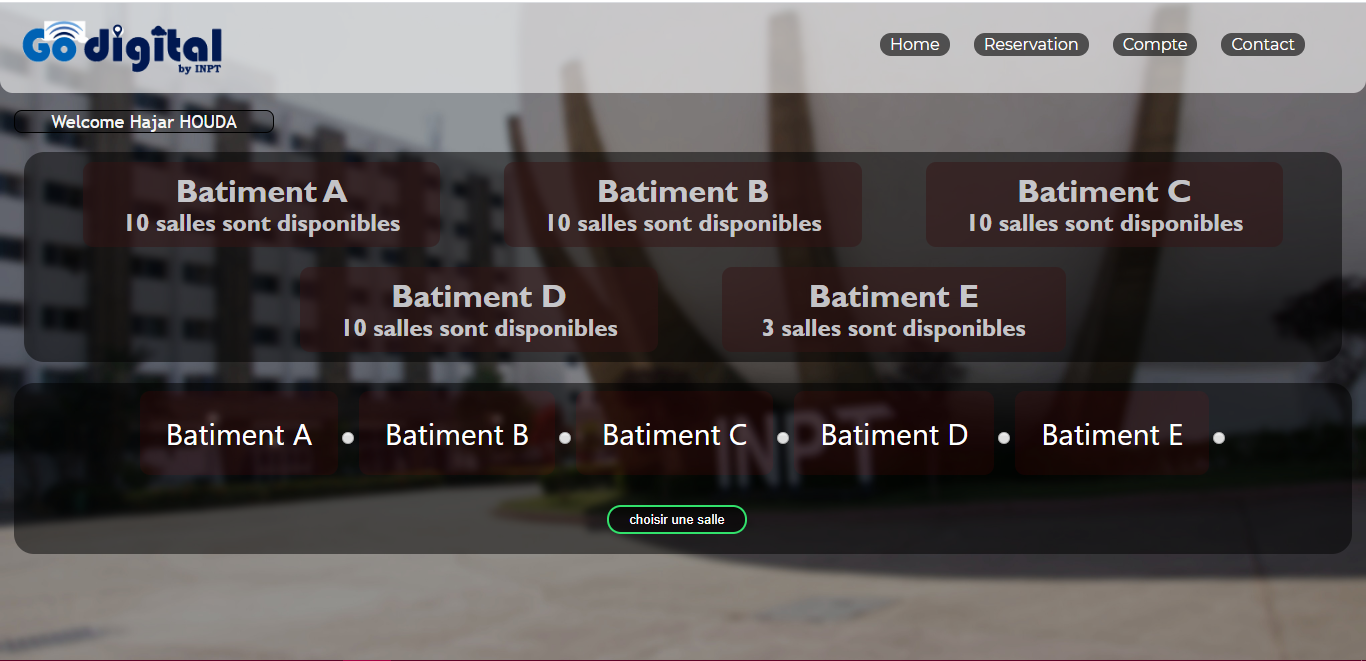
\includegraphics[width=18.8cm,height=8.5cm]{img/reservation.png}}  
  
  après avoir choisi un batiment, la page du formulaire est la suivante
  
  
  \vspace{0.7cm}
   
\hspace*{-0.7in}
               \noindent\makebox[\textwidth]{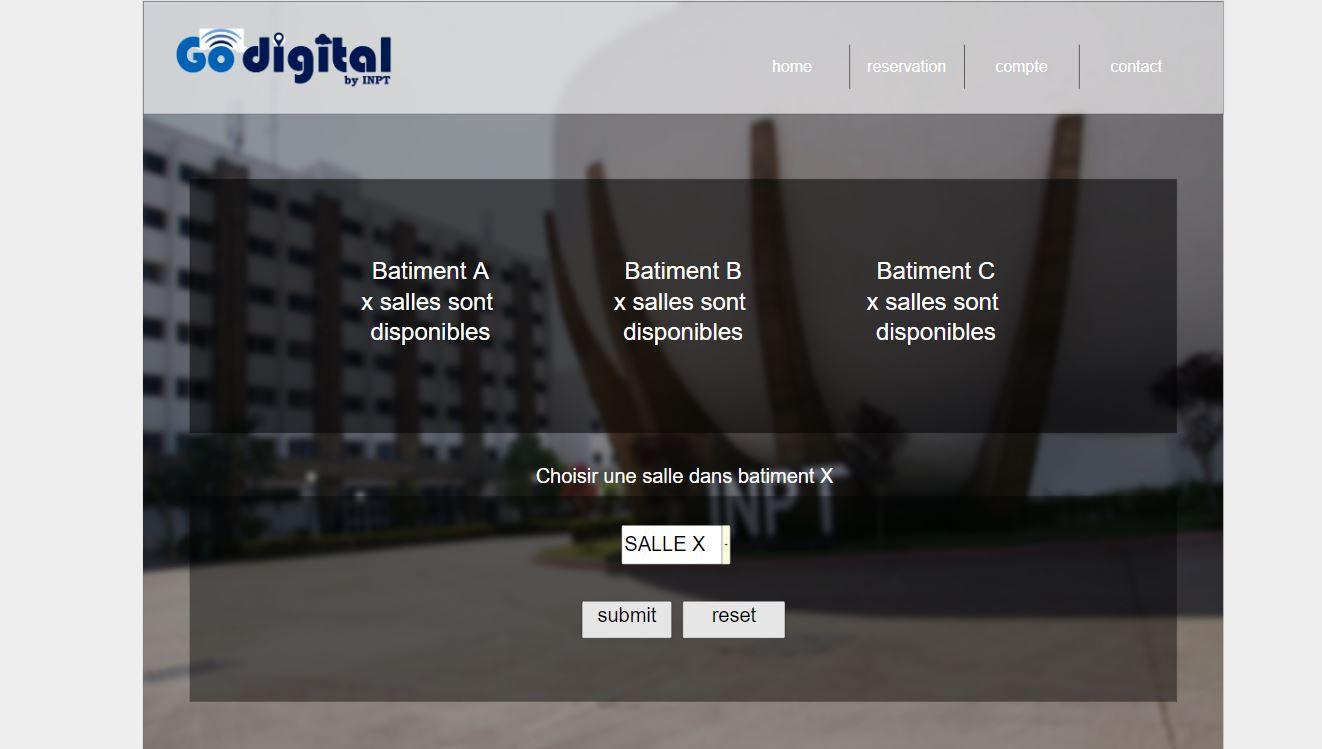
\includegraphics[width=18.8cm,height=8.5cm]{img/form.png}}   
  
  les options de sélection contiennent les salles dans le batiment choisi. Si la salle est déjà réservée, les options sont comme 'The first reservation of SALLX is ****/**/** **-**-**', sinon l'option est le nom de salle.
  
  \vspace{0.7cm}
   
\hspace*{-0.7in}
               \noindent\makebox[\textwidth]{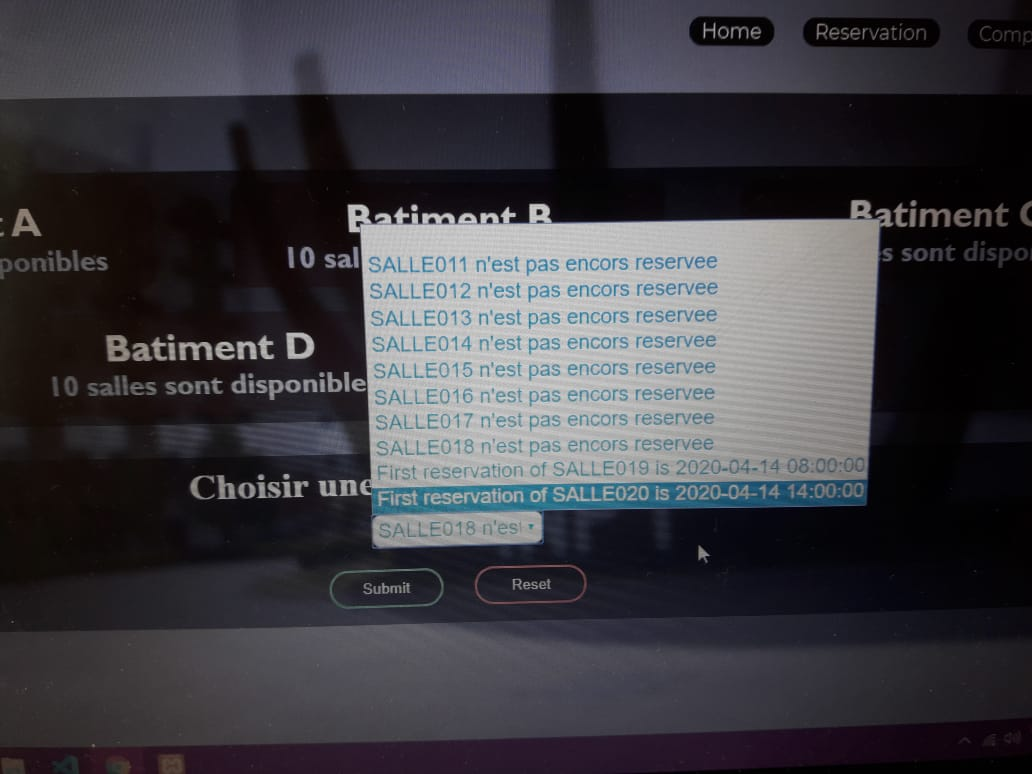
\includegraphics[width=18.8cm,height=8.5cm]{img/form-select.jpeg}}  
  
  
  Si vous sélectionnez une salle qui est déjà réservée, la page de réservation de date affiche son contenu comme l'image suivante qui montre les dates qui sont deja prises
  
  
  
  \vspace{0.7cm}
   
\hspace*{-0.7in}
               \noindent\makebox[\textwidth]{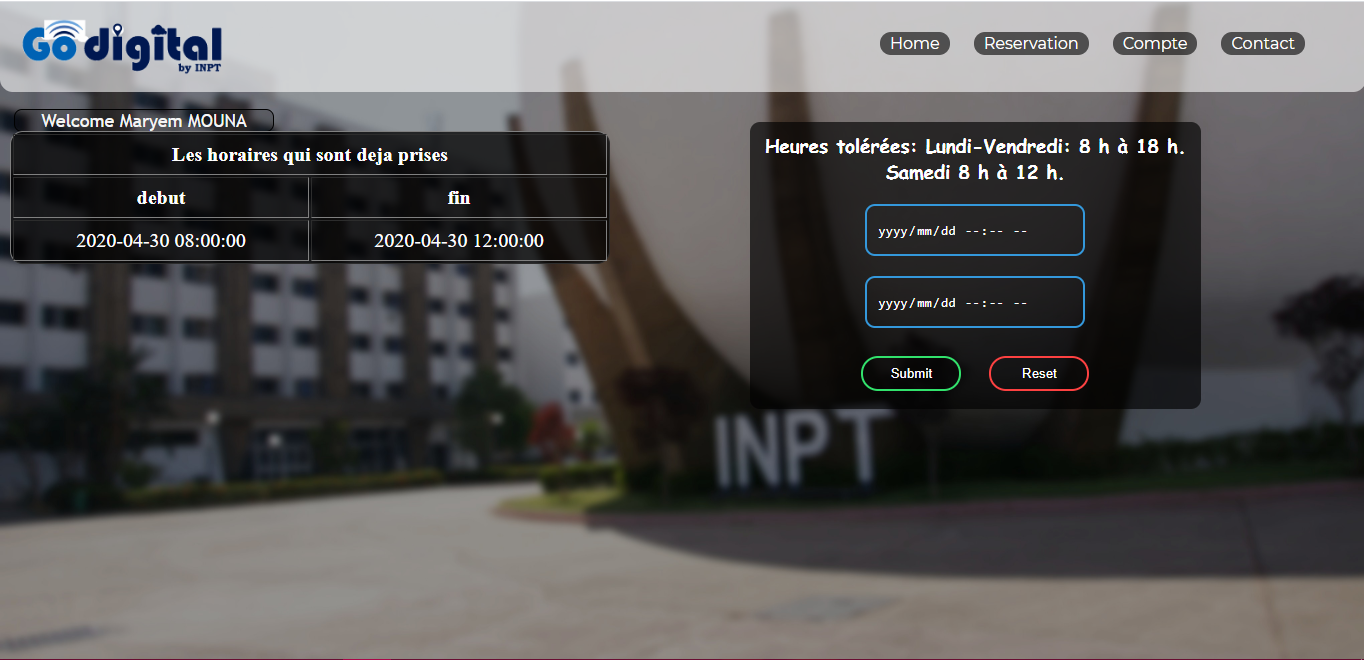
\includegraphics[width=18.8cm,height=8.5cm]{img/date-already.png}}  
  
  sinon cela se présente comme suit
  
  
  
               \vspace{0.7cm}
               \hspace*{-0.7in}
               \noindent\makebox[\textwidth]{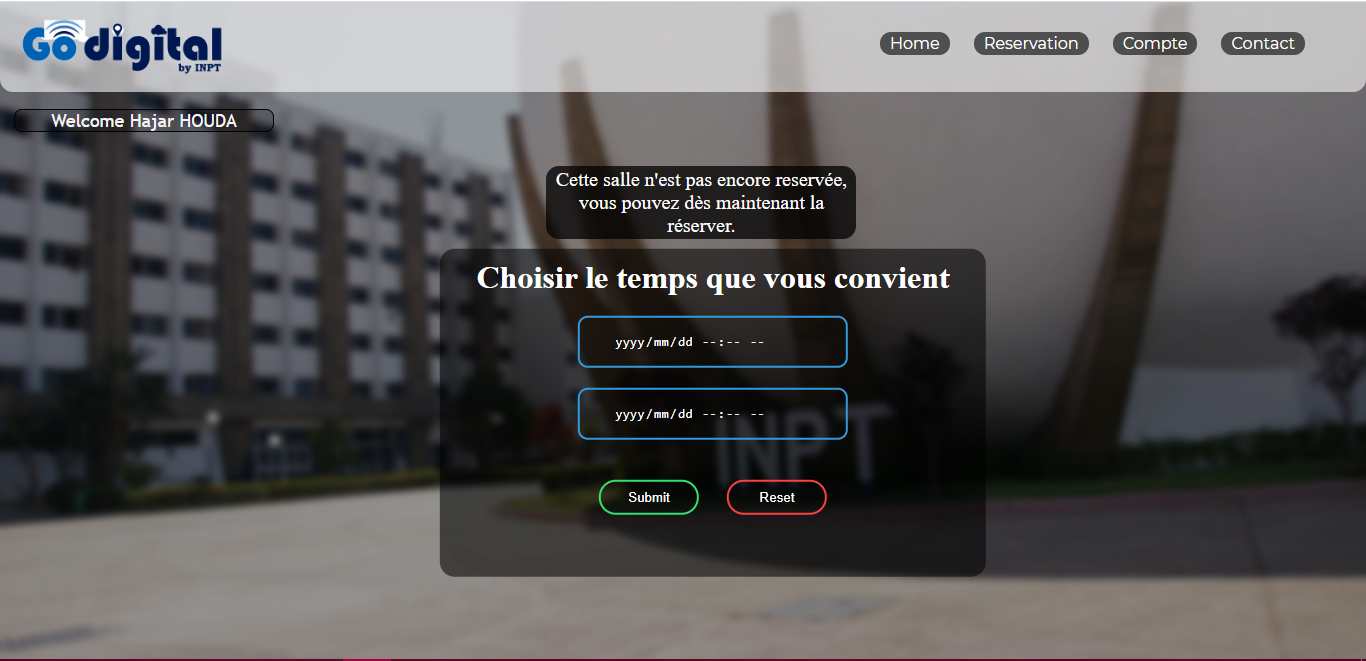
\includegraphics[width=18.8cm,height=8.5cm]{img/date-not-yet.png}}
  
  
  
  
  Maintenant, la boîte d'alerte affichera plusieurs messages en fonction des dates entrées par l'utilisateur. Pour un champ vide, le message d'alerte est le même que d'habitude. Il y a sept messages qui peuvent apparaître :
  
  \begin{enumerate}
 
 
  \item \textcolor{red}{les dates sont égales :} 
  \vspace{0.7cm}
               \hspace*{-0.7in}

               \noindent\makebox[\textwidth]{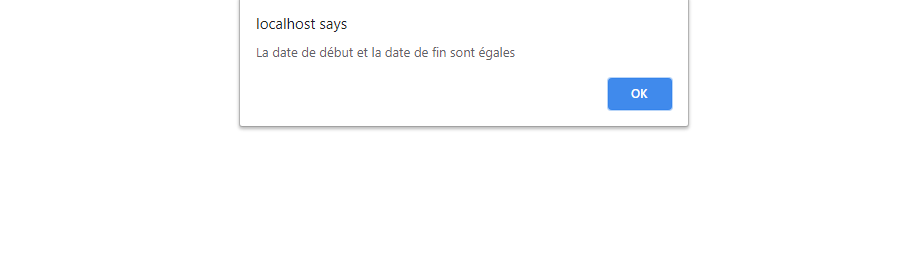
\includegraphics[width=18.8cm,height=8.5cm]{img/date-equal.png}}
               \newpage
  \item \textcolor{red}{les dates sont anciennes :} 
  \vspace{0.7cm}
               \hspace*{-0.7in}

               \noindent\makebox[\textwidth]{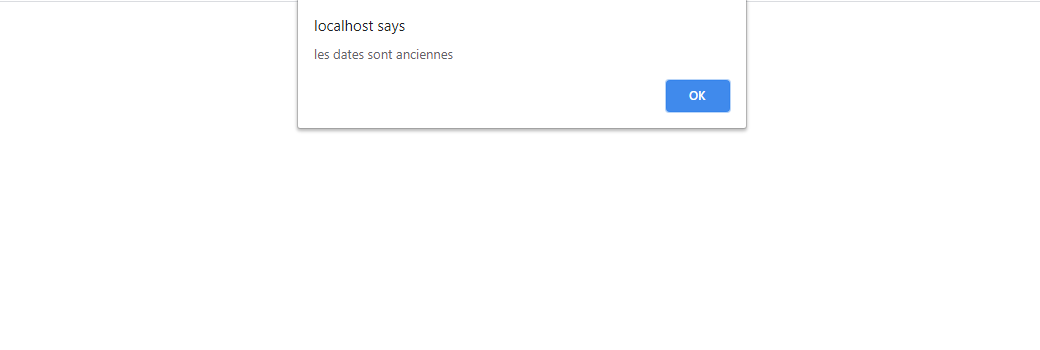
\includegraphics[width=18.8cm,height=5cm]{img/date-old.png}}
  \item \textcolor{red}{la durée de la réservation est courte :} 
  \vspace{0.7cm}
               \hspace*{-0.7in}

               \noindent\makebox[\textwidth]{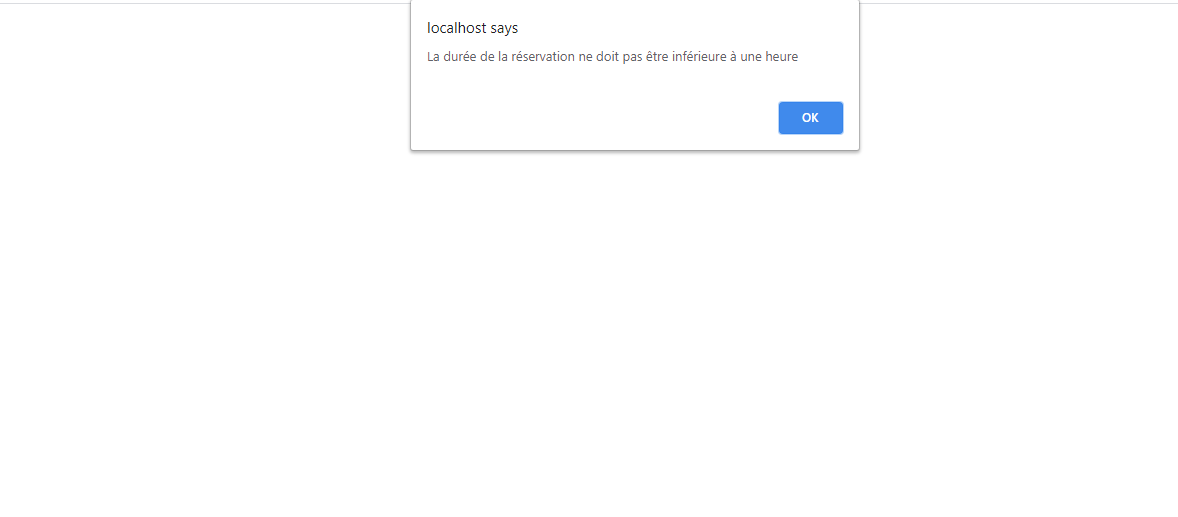
\includegraphics[width=18.8cm,height=5cm]{img/date-inferior.png}}
  \item \textcolor{red}{la durée de la réservation est longue :} 
  \vspace{0.7cm}
               \hspace*{-0.7in}

               \noindent\makebox[\textwidth]{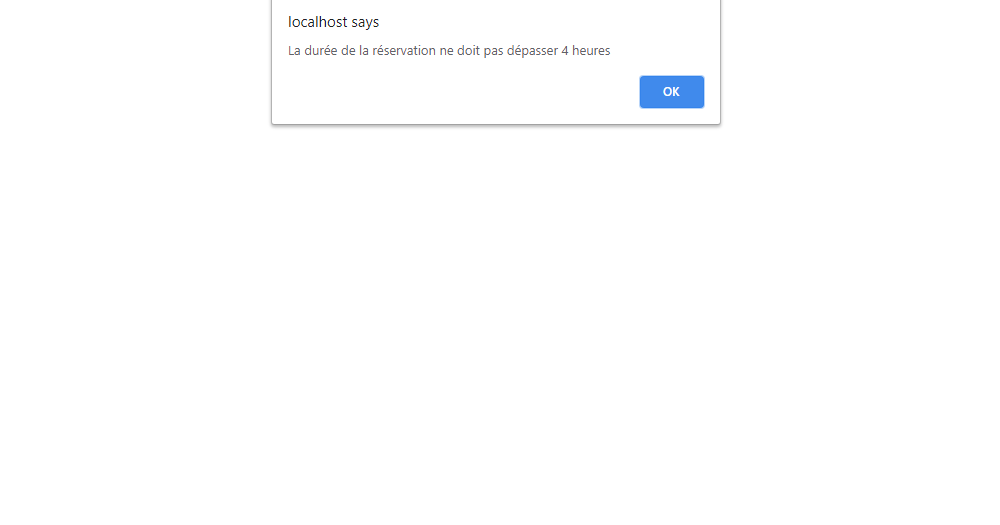
\includegraphics[width=18.8cm,height=5cm]{img/date-superior.png}}
  \item \textcolor{red}{les dates se croisent avec une autre date :} 
  \vspace{0.7cm}
               \hspace*{-0.7in}

               \noindent\makebox[\textwidth]{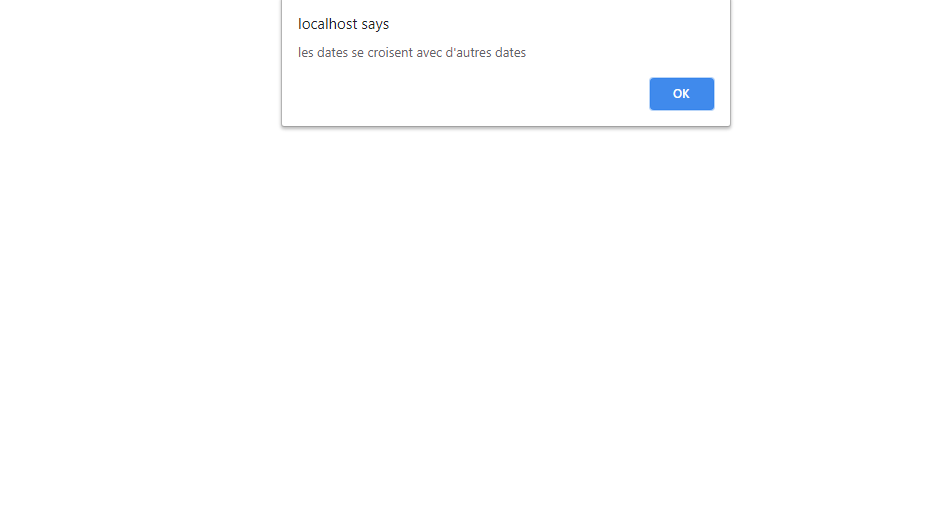
\includegraphics[width=18.8cm,height=5cm]{img/date-intersect.png}}
               
          \item \textcolor{red}{des heures qui ne sont pas comprises entre 8h00 et 18h00:}     
 \vspace{0.7cm}
               \hspace*{-0.7in}

               \noindent\makebox[\textwidth]{\includegraphics[width=18.8cm,height=5cm]{img/date-OutOfRange.png}} 
          
          
          \vspace{2.7cm}     
               \item \textcolor{red}{Le jour choisi est dimanche:}     
 \vspace{0.7cm}
               \hspace*{-0.7in}

               \noindent\makebox[\textwidth]{\includegraphics[width=18.8cm,height=5cm]{img/sunday.png}}          
          
          
          
          
          
               
  \item \textcolor{red}{les dates sont correctes :} 
  \vspace{0.3cm}
               \hspace*{-0.7in}

               \noindent\makebox[\textwidth]{\includegraphics[width=18.8cm,height=5cm]{img/date-done.png}}
  
\end{enumerate}  

Lorsque l'utilisateur effectue une réservation, un e-mail sera envoyé à l'administrateur comme l'image suivante montre :

\vspace{0.7cm}
               \hspace*{-0.7in}

               \noindent\makebox[\textwidth]{\includegraphics[width=18.8cm,height=8.5cm]{img/gmail-reservaton.jpg}}  
  
  
  
	Maintenant, après avoir fait la réservation, le dernier apparaîtra avec un tableau qui montre votre réservation et vous ne pourrez plus visiter la page de choix des salles, des batiments ou des dates. Si vous cliquez sur le bouton Annuler, la boîte d'alerte de confirmation apparaîtra pour vous demander votre confirmation, si vous confirmez que votre réservation sera supprimée.
  
  \vspace{0.7cm}
               \hspace*{-0.7in}
               \noindent\makebox[\textwidth]{\includegraphics[width=18.8cm,height=8.5cm]{img/reservation-annuler.png}}
  
  
Lorsque l'utilisateur annule sa réservation, un e-mail sera envoyé à l'administrateur comme l'image suivante montre :  
  
	\vspace{0.7cm}
               \hspace*{-0.7in}
               \noindent\makebox[\textwidth]{\includegraphics[width=18.8cm,height=8.5cm]{img/gmail-annulation.jpg}}  
  
  
  
  
  
  
  
  
  
  
Maintenant, si l'administrateur s'est connecté, les pages d'accueil contiendront un autre lien au lieu de la scène de la page de contact, c'est inutile pour le cas.
  
  
  
  \vspace{0.7cm}
               \hspace*{-0.7in}
               \noindent\makebox[\textwidth]{\includegraphics[width=18.8cm,height=8.5cm]{img/home-admin.png}}
  
  
  La page de modification de l'utilisateur affiche un tableau avec toutes les informations sur les utilisateurs et le côté gauche contient un formulaire pour ajouter ou supprimer un utilisateur.
  
  
  
  \vspace{0.7cm}
               \hspace*{-0.7in}
               \noindent\makebox[\textwidth]{\includegraphics[width=18.8cm,height=8.5cm]{img/modify.png}}
  
  
  Si l'administrateur souhaite ajouter un utilisateur:
  
  
   
  \vspace{0.7cm}
               \hspace*{-0.7in}
               \noindent\makebox[\textwidth]{\includegraphics[width=18.8cm,height=8.5cm]{img/modify-add.png}}
  
  
   Puis après avoir accepté:
  
  \vspace{0.7cm}
               \hspace*{-0.7in}

               \noindent\makebox[\textwidth]{\includegraphics[width=18.8cm,height=7cm]{img/modify-added.PNG}}
  
  
  
  Supposons maintenant que nous voulions supprimer l'utilisateur Mohamed ABDELLAH, on click sur la boutton supprimer.
  
  le bouton d'alerte attend notre confirmation
  
\vspace{0.7cm}
               \hspace*{-0.7in}

               \noindent\makebox[\textwidth]{\includegraphics[width=18.8cm,height=7cm]{img/modify-remove-accept.png}}  
  
  \vspace{2cm}
  Puis après avoir accepté:
  
  \vspace{0.7cm}
               \hspace*{-0.7in}

               \noindent\makebox[\textwidth]{\includegraphics[width=18.8cm,height=7cm]{img/modify-removed.png}}
  
  Supposons maintenant que nous voulions activer un utilisateur dont la réinitialisation du mot de passe a été bloquée :
  le bouton d'alerte attend notre confirmation
  \vspace{0.7cm}
               \hspace*{-0.7in}

               \noindent\makebox[\textwidth]{\includegraphics[width=18.8cm,height=7cm]{img/wanna-activate.PNG}}
  
   Puis après avoir accepté:
  
  \vspace{0.7cm}
               \hspace*{-0.7in}

               \noindent\makebox[\textwidth]{\includegraphics[width=18.8cm,height=7cm]{img/user-activated.PNG}}
  
  
  
  \newpage 
  La page d'affectation affiche toutes les réservations des utilisateurs, mais celle de l'administrateur apparaîtra en rouge :
  
  \vspace{0.7cm}
               \hspace*{-0.7in}
               \noindent\makebox[\textwidth]{\includegraphics[width=18.8cm,height=8.5cm]{img/affectation.png}}
               
               
    \vspace{4cm}           
               Maintenant, si vous restez inactif pendant 15 minutes, la session sera expirera automatiquement. La boîte d'alerte est comme suit
  
 \vspace{0.7cm}
               \hspace*{-0.7in}
               \noindent\makebox[\textwidth]{\includegraphics[width=18.8cm,height=8.5cm]{img/expired-session.png}}  
  
  
  
  
  
  
	\vspace{3cm}
 \item \textcolor{red}{\huge Choses non fonctionnelles} :  
   \vspace{0.7cm}
        
        \begin{enumerate}
        \item\textcolor{blue}{Empêcher l'accès direct aux pages Web}
        \item\textcolor{blue}{Empêcher l'accès direct aux pages Web d'administration}
        \item\textcolor{blue}{Empêcher l'accès aux répertoires de l'application Web}
        \item\textcolor{blue}{Empêcher la réinitialisation du mot de passe après 10 tentatives infructueuses}
        \item\textcolor{blue}{Empêcher l'accès direct à certaines pages sans passer par des pages}
        
        
        \end{enumerate} 
  
  Il y a certaines pages auxquelles les utilisateurs ne peuvent pas accéder à moins qu'ils ne soient l'administrateur, donc si l'utilisateur essaie d'entrer dans ces pages la boîte d'alerte lui donnera un message comme l'image suivante s'affiche et juste après cela, la session sera automatiquement détruite.
  
   
  
\vspace{0.7cm}
               \hspace*{-0.7in}
               \noindent\makebox[\textwidth]{\includegraphics[width=18.8cm,height=8.5cm]{img/cant-access.png}} 



Si l'utilisateur n'a pas saisi le bon code de réinitialisation du mot de passe 10 fois, il n'est plus en mesure de réinitialiser le mot de passe pour les deux prochaines heures.



  
\vspace{0.7cm}
               \hspace*{-0.7in}
               \noindent\makebox[\textwidth]{\includegraphics[width=18.8cm,height=8.5cm]{img/ten-attempts.png}} 


Et quand il reviendra après avoir reçu ce message avec le même e-mail, il recevra le message suivant :

\vspace{0.7cm}
               \hspace*{-0.7in}
               \noindent\makebox[\textwidth]{\includegraphics[width=18.8cm,height=8.5cm]{img/after-block.PNG}} 



\vspace{0.7cm}
Maintenant, chaque dossier du site Web est protégé contre l'accès par le fichier \textcolor{red}{htaccess}, lorsque vous essayez d'accéder dans ce cas, le serveur vous empêchera de le faire

\hspace*{-0.7in}
               \noindent\makebox[\textwidth]{\includegraphics[width=18.8cm,height=8.5cm]{img/htaccess.png}} 


 
  
  \vspace{3cm}
\item \textcolor{red}{\huge Les problèmes rencontrés dans mon projet} :
\begin{enumerate}
\item    \textcolor{green}{ GMAIL et PHP} :

   \vspace{0.4cm}
                \setlength{\parindent}{1cm} Je n'ai pas réussi à effectuer certaines tâches complètement. Concernant le formulaire de contact, \textcolor{blue}{\textbf{GMAIL}} bloque tout message envoyé par \textcolor{blue}{\textbf{PHP}}, elles sont traités comme du spam. Mais l'application \textcolor{blue}{\textbf{PHPMAILER}} n'ai pas réussi à envoyer des mails à mon compte  comme le montre l'image suivante :
   
   \vspace{0.6cm}
   \hspace*{-1.05in}
               \noindent\makebox[\textwidth]{\includegraphics[width=14cm,height=6cm]{img/gmail-block.PNG}}
               \vspace{0.4cm}
               Mais la solution est que je envoie un message d'un compte gmail, mon compte, à un qui aussi mon compte mais le message va contenir ce que l'utilisateur a saisie.
  
    \vspace{4cm}
    
    \item    \textcolor{green}{ XAMPP et HTACCESS} :
    
    \vspace{0.4cm}
                \setlength{\parindent}{1cm} Pour crypter les fichiers et dossiers qui contiennent des informations privées sur mon site Web, j'avais besoin d'utiliser le fichier \textcolor{blue}{\textbf{htaccess}}. Le fichier \textcolor{blue}{\textbf{htaccess}} est détecté et exécuté par le logiciel Apache Web Server, mais dans mon cas, \textcolor{blue}{\textbf{XAMPP}} ne peut pas exécuter le fichier \textcolor{blue}{\textbf{htaccess}}. L'image suivante montre l'erreur obtenue lors de la tentative d'entrer dans un fichier ou un dossier crypté :
    
    \vspace{1cm}

 \hspace*{-1.05in}
               \noindent\makebox[\textwidth]{\includegraphics[width=16cm,height=7cm]{img/ht-error.PNG}}
  
   \vspace{0.6cm}  
	\textcolor{red}{\huge \warning} Comme vous le voyez sur l'image même si j'entre le nom d'utilisateur et le mot de passe correct le serveur n'arrive pas à me laisser entrer dans ce dossier.  
  \end{enumerate}
  
 
  
  \vspace{3cm} 
\item  \textcolor{red}{\Huge Remerciements} :   
  \vspace{2cm} 
  
\setlength{\parindent}{1cm}  \huge	Je tiens vraiment à remercier M. ELHAMLAOUI qui nous a donné son temps pour nos questions
					\linebreak  et pour nous aider pendant nos études en classe
					\linebreak  ainsi qu'en ligne, La méthode de travail \linebreak qu'il a suggérée  m'a vraiment plu,\linebreak car cela  m'aidera à travailler  facilement avec \linebreak d'autres 
					  personnes dans le future.
  
  
  
\end{enumerate}


\end{document}
